% !TeX encoding = UTF-8
% !TeX program = xelatex
% !TeX spellcheck = en_US

\documentclass[degree=master,language=chinese,font=external,cjk-font=external]{sustechthesis}
  %%%%%%%%%%%%%%%%%%%%%%%%%%%%%%%%%%%%%%%
  %   研究生报告模板:开题报告,年度考核报告
  %%%%%%%%%%%%%%%%%%%%%%%%%%%%%%%%%%%%%%%

  % 学位 degree:
  %   master (默认) | doctor
  % 语言 language:
  %   chinese (默认)| english
  % 英文字体 font
  %   auto (默认,自动选择系统自带字体)| external (包内字体)| times | termes | 等
  %   Windows 和 macOS 系统上,无需设定。系统自带对应字体,可以删除该参数。
  %   Unix 系统推荐使用包内字体,而非TeX自带的克隆版字体,以达到和其他系统一致的字体效果。
  %   Windows 系统上可以删除该参数,使用系统内置字体。
  % 中文字体 cjk-font
  %   auto (默认,自动选择系统自带字体)| external (包内字体)| windows | mac | 等
  %   在 **非Windows** 的系统上推荐使用包内字体,而非系统字体。
  %   以达到和 Windows 系统一致的字体效果。
  %   Windows 系统自带对应字体,可以删除该参数。

  
% 论文基本配置,加载宏包等全局配置
% 在此文件中可以选择
% 1. 【重要】文档类型(开题报告,年度考核报告),默认不开启该选项。
% 2. 生成的PDF为无空白页的用于电子版提交的版本 或 插入空白页的以便双面打印的版本
% 3. 学位学科门类(理学、工学、医学)
% 4. 培养单位
% 5. 作者姓名、指导教师等
% !TeX root = ./sustechthesis-example.tex

% 论文基本信息配置

\thusetup{
  %******************************
  % 注意:
  %   1. 配置里面不要出现**空行**
  %   2. 不需要的配置信息可以删除
  %   3. 建议先阅读文档中所有关于选项的说明
  %******************************
  %
  % 输出格式
  %   选择打印版(print)或用于提交的电子版(electronic),前者会插入空白页以便直接双面打印
  %
  output = print,
  %
  % 文档类型
  %   选择开题报告(proposal)、年度考核报告(progress)或学位论文(thesis)【默认值】。
  %
  type = thesis,
  %
  % 标题
  %   可使用“\\”命令手动控制换行
  %   如果需要使用副标题,取消 subtitle 和 subtitle* 的注释即可。
  %   特别字符允许小写,例如行内公式,其他所有字词全部大写。
  %
  title  = {脉冲激光实现离子量子比特门},
  title* = {Implementation of ion-qubit gate by pulsedlaser},
  % subtitle = {可选的副标题可选的副标题可选的副标题可选的副标题可选的副标题可选的副标题},
  % subtitle* = {optional subtitle optional subtitle optional subtitle optional subtitle optional subtitle optional subtitle},
  %
  % 学位
  %
  degree-domain = {工学}, % 【中文】学科门类:可选理学、工学、医学
  degree-domain* = {Engineering}, % 【英文】学位等级:可选Science, Engineering, Medicine
  gongshuo = false, % 是否为专业型学位。专业型学位则填 true ,学术型或其他为 false 。
  %
  % 培养单位
  %   填写所属院系的全名
  %   超长英文系名可以手动换行
  department = {量子科学与工程研究院},
  department* = {Institute of Quantum Science and Engineering},
  %
  % 学科
  %   1. 学术型学位
  %      获得一级学科授权的学科填写一级学科名称,其他填写二级学科名称
  %   2. 工程硕士
  %      工程领域名称
  %
  discipline  = {电子科学与技术},
  discipline* = {Electronic Science and Technology},
  %
  % 姓名
  %   英文用全拼,姓在前,名在后,姓和名的首字母大写,其余小写
  %
  author-id  = {12132850},
  author  = {彭道杰},
  author* = {PENG Daojie},
  %
  % 指导教师
  %   一般情况下,只写一名指导教师。
  %   填写导师姓名,后衬导师职称“教授”,“副教授”,“研究员”等
  %
  supervisor  = {张君华副研究员},
  supervisor* = {Assistant Researcher ZHANG Junhua},
  % 副指导教师
  %   一般无需启用该项,留空或者注释掉即可。
  %   如需启用限填写一名,且需要向学位办确认和备案,职称要求同指导教师。
  % associate-supervisor  = {大卫查理助理教授},
  % associate-supervisor* = {Assistant Prof. David Charlie},
  %
  % 日期
  %   使用 ISO 格式;默认为当前时间
  %   date 为第一页全中文大写日期,defense-date 为第二、三页的答辩日期。
  %   需要按 {年-月-日} 格式填写,如不显示“日”,可以随意填一个日期,但是不能为空。
  %
  date = {2024-3-1},
  defense-date = {2024-4-1},
  %
  % 密级
  %   公开, 秘密, 机密, 绝密
  %
  statesecrets={公开},
  %
  % 国内图书分类号:查询网址:https://ztflh.xhma.com/
  %   国内图书分类号可先参考知网上类似学位论文的分类号,再进行确认。
  % 国际图书分类号,查询网址:https://udcsummary.info/php/index.php?lang=chi
  %
  natclassifiedindex={XXxxx.x},
  intclassifiedindex={xx-x},
}

\thusetup{
  %
  % 数学字体
  % math-style = GB,  % GB (中文默认) | TeX (英文默认)
  math-font  = cambria,  % cambria (默认,同 Word 默认数学字体一致) | times (Times New Roman 的TeX克隆版)| xits | stix
}

% 载入所需的宏包

% 可以使用 nomencl 生成符号和缩略语说明
% \usepackage{nomencl}
% \makenomenclature

% 表格加脚注
\usepackage{threeparttable}

% 表格中支持跨行
\usepackage{multirow}

% 量和单位
\usepackage{siunitx}

% 定理类环境宏包
\usepackage{amsthm}
% 也可以使用 ntheorem
% \usepackage[amsmath,thmmarks,hyperref]{ntheorem}

%%%%%% 顺序编码制的文献引用形式
%%%%%% 参考文献编译方式二选一,不要同时开启。
%%%% 选择一:使用 BibTeX + natbib 宏包
\usepackage[sort&compress]{gbt7714}
\citestyle{super} % 全局上标数字模式
% \citestyle{numbers} % 全局行内数字模式,在写作指南2022年8月23日版本已废弃, 并决定中英文都采用上标数字格式
\bibliographystyle{sustechthesis-numeric}

%%%% 选择二:使用 BibLaTeX 宏包(兼容性不佳,不太推荐)
% \usepackage[backend=biber,style=gb7714-2015,gbalign=left]{biblatex}
% \addbibresource{ref/refs.bib} % 声明 BibLaTeX 的数据库

% 定义所有的图片文件在 figures 子目录下
\graphicspath{{figures/}}

% 数学命令
\newcommand\dif{\mathop{}\!\mathrm{d}}  % 微分符号

% hyperref 宏包在最后调用
\usepackage{hyperref}
\usepackage{ragged2e}

% 固定宽度的表格。放在 hyperref 之前的话,tabularx 里的 footnote 显示不出来。
\usepackage{tabularx}

% 跨页表格,必须在 hyperref 之后使用否则会报错。
\usepackage{longtable}

% % 源代码 minted 高亮,二选一即可。【不再推荐,会有兼容性问题:导致图表间距异常】
% %% 使用 minted 包有内置高亮颜色,需要 Python 环境编译,并安装 Pygement 包。
% \usepackage{minted}

% 源代码 listings 高亮,二选一即可。
\usepackage{listings}
%% 使用 listings 包需要自行定义高亮颜色,此处给出 Java 的例子。
\definecolor{javared}{rgb}{0.6,0,0} % for strings
\definecolor{javagreen}{rgb}{0.25,0.5,0.35} % comments
\definecolor{javapurple}{rgb}{0.5,0,0.35} % keywords
\definecolor{javadocblue}{rgb}{0.25,0.35,0.75} % javadoc

\lstset{language=Java,
  keywordstyle=\color{javapurple}\bfseries,
  stringstyle=\color{javared},
  commentstyle=\color{javagreen},
  morecomment=[s][\color{javadocblue}]{/**}{*/},
  numbers=left,
  numberstyle=\tiny\color{black},
  stepnumber=1,
  numbersep=10pt,
  tabsize=4,
  showspaces=false,
  showstringspaces=false
}

% 伪代码环境
\usepackage[ruled,linesnumbered]{algorithm2e}
% 定义伪代码的continue
\SetKw{Continue}{continue}
\SetKw{Break}{break}
% 定义算法注释
\SetKwComment{Comment}{/* }{ */}
\SetKwComment{SingleComment}{// }{}
\SetKwComment{TriComment}{$\triangleright$\ }{}

% tabular 扩展命令
\newcolumntype{R}[1]{>{\raggedleft\arraybackslash}p{#1}} % 定义R为表格左右居左,用于自定义表格列宽度
\newcolumntype{L}[1]{>{\raggedright\arraybackslash}p{#1}} % 定义L为表格左右居右,用于自定义表格列宽度
\newcolumntype{C}[1]{>{\centering\arraybackslash}p{#1}} % 定义C为表格左右居中,用于自定义表格列宽度

% tabularx 扩展命令,会对单元格内容进行单元格内自动换行
% X 默认就是两端对齐
% Y 左对齐
\newcolumntype{Y}{>{\raggedright\arraybackslash}X}
% Z 右对齐
\newcolumntype{Z}{>{\raggedleft\arraybackslash}X}
% A 居中对齐
\newcolumntype{A}{>{\centering\arraybackslash}X}

% 表格旋转
\usepackage{rotating}


\newcommand\undefcolumntype[1]{\expandafter\let\csname NC@find@#1\endcsname\relax}
\newcommand\forcenewcolumntype[1]{\undefcolumntype{#1}\newcolumntype{#1}}


\begin{document}

% 封面
\maketitle

\frontmatter

% 目录
\tableofcontents

% 插图和附表清单
% \listoffiguresandtables  % 插图和附表清单
% \listoffigures           % 插图清单
% \listoftables            % 附表清单

% 符号对照表(非强制性要求,如果论文中所用符号不多,可以略去)
% % !TeX root = ../sustechthesis-example.tex

% denotation 环境带一个可选参数,用来指定符号列的宽度(默认为 2.5cm),下面改3cm为例。
% 如果论文中使用了大量的物理量符号、标志、缩略词、专门计量单位、自定义名词和术语等, 应编写“符号和缩略语说明”。
% 论文中主要符号应全部采用法定单位, 严格执行《量和单位》(GB3100~3102-93)的有关规定、单位名称的书写,可以采用国际通用符号,也可以用中文名称,但全文应统一,不得两种混用。
% 缩略语应列出中英文全称。符号和缩略语说明排序方法先按拉丁字母大写、小写排序, 再按希腊字母大写、小写排序, 如下表所示:
% ABCDEFGHIJKLMNOPQRSRUVWXYZ
% abcdefghijklmnopqrstuvwxyz
% Alpha
% Beta
% Gamma
% Delta
% Epsilon
% Zeta
% Eta
% Theta
% Iota
% Kappa
% Lambda
% Mu
% Nu
% Xi
% Omicron
% Pi
% Rho
% Sigma
% Tau
% Upsilon
% Phi
% Chi
% Psi
% Omega
% alpha
% beta
% gamma
% delta
% epsilon
% zeta
% eta
% theta
% iota
% kappa
% lambda
% mu
% nu
% xi
% omicron
% pi
% rho
% sigma
% tau
% upsilon
% phi
% chi
% psi
% omega

% 希腊字母详见 https://xilazimu.net/


\begin{denotation}[3cm]
  \item[RF] 射频(Radio Frequency)
  \item[PQS] 量子叠加原理(Principle of Quantum Superposition)
  \item[DCT] 动态解耦技术(Dynamic Decoupling Technology)
  \item[UQC] 通用量子计算机(Universal Quantum Computer)
\end{denotation}



% 也可以使用 nomencl 宏包,需要在导言区
% \usepackage{nomencl}
% \makenomenclature

% 在这里输出符号说明
% \printnomenclature[3cm]

% 在正文中的任意为都可以标题
% \nomenclature{As-PPT}{聚苯基不对称三嗪}
% \nomenclature{DFT}{密度泛函理论 (Density Functional Theory)}
% \nomenclature{DMAsPPT}{聚苯基不对称三嗪双模型化合物(水解实验模型化合物)}
% \nomenclature{$E_a$}{化学反应的活化能 (Activation Energy)}
% \nomenclature{HMAsPPT}{聚苯基不对称三嗪模型化合物的质子化产物}
% \nomenclature{HMPBI}{聚苯并咪唑模型化合物的质子化产物}
% \nomenclature{HMPI}{聚酰亚胺模型化合物的质子化产物}
% \nomenclature{HMPPQ}{聚苯基喹噁啉模型化合物的质子化产物}
% \nomenclature{HMPY}{聚吡咙模型化合物的质子化产物}
% \nomenclature{HMSPPT}{聚苯基对称三嗪模型化合物的质子化产物}
% \nomenclature{HPCE}{高效毛细管电泳色谱 (High Performance Capillary lectrophoresis)}
% \nomenclature{HPLC}{高效液相色谱 (High Performance Liquid Chromatography)}
% \nomenclature{IRC}{内禀反应坐标 (Intrinsic Reaction Coordinates)}
% \nomenclature{LC-MS}{液相色谱-质谱联用 (Liquid chromatography-Mass Spectrum)}
% \nomenclature{MAsPPT}{聚苯基不对称三嗪单模型化合物,3,5,6-三苯基-1,2,4-三嗪}
% \nomenclature{MPBI}{聚苯并咪唑模型化合物,N-苯基苯并咪唑}
% \nomenclature{MPI}{聚酰亚胺模型化合物,N-苯基邻苯酰亚胺}
% \nomenclature{MPPQ}{聚苯基喹噁啉模型化合物,3,4-二苯基苯并二嗪}
% \nomenclature{MPY}{聚吡咙模型化合物}
% \nomenclature{MSPPT}{聚苯基对称三嗪模型化合物,2,4,6-三苯基-1,3,5-三嗪}
% \nomenclature{ONIOM}{分层算法 (Our own N-layered Integrated molecular Orbital and molecular Mechanics)}
% \nomenclature{PBI}{聚苯并咪唑}
% \nomenclature{PDT}{热分解温度}
% \nomenclature{PES}{势能面 (Potential Energy Surface)}
% \nomenclature{PI}{聚酰亚胺}
% \nomenclature{PMDA-BDA}{均苯四酸二酐与联苯四胺合成的聚吡咙薄膜}
% \nomenclature{PPQ}{聚苯基喹噁啉}
% \nomenclature{PY}{聚吡咙}
% \nomenclature{S-PPT}{聚苯基对称三嗪}
% \nomenclature{SCF}{自洽场 (Self-Consistent Field)}
% \nomenclature{SCRF}{自洽反应场 (Self-Consistent Reaction Field)}
% \nomenclature{TIC}{总离子浓度 (Total Ion Content)}
% \nomenclature{TS}{过渡态 (Transition State)}
% \nomenclature{TST}{过渡态理论 (Transition State Theory)}
% \nomenclature{ZPE}{零点振动能 (Zero Vibration Energy)}
% \nomenclature{\textit{ab initio}}{基于第一原理的量子化学计算方法,常称从头算法}
% \nomenclature{$\Delta G^\neq$}{活化自由能(Activation Free Energy)}
% \nomenclature{$\kappa$}{传输系数 (Transmission Coefficient)}
% \nomenclature{$\nu_i$}{虚频 (Imaginary Frequency)}



% 正文部分
\mainmatter
% !TeX root = ../sustechthesis-example.tex

\chapter{论文主要部分的写法}

研究生学位论文撰写,除表达形式上需要符合一定的格式要求外,内容方面上也要遵循一些共性原则。

通常研究生学位论文只能有一个主题(不能是几块工作拼凑在一起),该主题应针对某学科领域中的一个具体问题展开深入、系统的研究,并得出有价值的研究结论。
学位论文的研究主题切忌过大,例如,“中国国有企业改制问题研究”这样的研究主题过大,因为“国企改制”涉及的问题范围太广,很难在一本研究生学位论文中完全研究透彻。

正文主要包括论文的选题背景与目的,论文研究领域发展趋势的分析与述评,论文的选题立论,研究方案阐述,主要研究结果阐释,讨论与研究展望,结论。此部分是论文的主体, 打印时应从另页右页开始,电子版与打印版每一章应另起页。主体部分一般从引言(绪论)开始,以结论结束,分章节论述,层次分明、逻辑性强。

论文正文字数要求为:博士学位论文正文一般为6~10万字(含图表);硕士学位论文正文一般为3~5万字(含图表),如冲突以《南方科技大学研究生学位论文写作指南》为准。

Word count in a doctoral thesis is generally 45 to 50 thousand English words (including tables and figures). And word count in a master's thesis is enerally 22 to 25 thousand English words (including tables and figures). Where any discrepancy arises between this template and the \textit{Guide to thesis writing for graduate students}, the ``Guide'' shall prevail.


\section{论文的语言及表述}

学位论文一般需要用汉语书写。满足下列情况之一, 可以用英文撰写学位论文:

\begin{enumerate}
\item 研究生本身英文水平较高, 且导师为外籍教师或有海外留学或工作经验, 英语水平较高, 可以指导学生用英文撰写论文;
\item 研究生参加双学位国际联合培养项目;
\item 国际研究生。
\end{enumerate}

研究生必须经导师同意后, 方能申请用英文撰写学位论文, 在参加开题评议时需提交中文版开题报告及对应的英文版开题报告, 由开题评议小组对其英文写作水平进行把关, 并给予审核意见。使用英文撰写论文的研究生原则上应采用英文进行答辩。采用英文撰写时须采用中文封面, 且应有800-1000汉字(符)摘要。

中文学位论文,除古汉语研究中涉及的古文字和参考文献中引用的外文文献之外,均采用简体汉字撰写。

研究生学位论文是学术作品,因此其表述要严谨简明,重点突出,专业常识应简写或不写,做到立论正确、数据可靠、说明透彻、推理严谨、文字凝练、层次分明,避免使用文学性质的或带感情色彩的非学术性语言。

论文中如出现一个非通用性的新名词、新术语或新概念,需随即解释清楚。



\section{论文题目的写法}

论文题目应简明扼要地反映论文工作的主要内容,力求精炼、准确,切忌笼统。
论文题目是对研究对象的准确、具体描述,一般要在一定程度上体现研究结论,因此,论文题目不仅应告诉读者这本论文研究了什么问题,更要告诉读者这个研究得出的结论。
例如:“在事实与虚构之间:梅乐、卡彭特、沃尔夫的新闻观”就比“三个美国作家的新闻观研究”更专业、更准确。



\section{摘要的写法}

论文摘要是对论文研究内容的高度概括,应具有独立性和自含性,即应是 一篇简短但意义完整的文章。
通过阅读论文摘要,读者应该能够对论文的研究 方法及结论有一个整体性的了解,因此摘要的写法应力求精确简明。
论文摘要 应包括对问题及研究目的的描述、对使用的方法和研究过程进行的简要介绍、 对研究结论的高度凝练等,重点是结果和结论。

论文摘要切忌写成全文的提纲,尤其要避免“第 1 章……;第 2 章……;……”这样的陈述方式。



\section{引言的写法}

一篇学位论文的引言大致包含如下几个部分:
1、问题的提出;
2、选题背 景及意义;
3、文献综述;
4、研究方法;
5、论文结构安排。
\begin{itemize}
  \item 问题的提出:要清晰地阐述所要研究的问题“是什么”。
    % \footnote{选题时切记要有“问题意识”,不要选不是问题的问题来研究。}
  \item 选题背景及意义:论述清楚为什么选择这个题目来研究,即阐述该研究对学科发展的贡献、对国计民生的理论与现实意义等。
  \item 文献综述:对本研究主题范围内的文献进行详尽的综合述评,“述”的同时一定要有“评”,指出现有研究状态,仍存在哪些尚待解决的问题,讲出自己的研究有哪些探索性内容。
  \item 研究方法:讲清论文所使用的学术研究方法。
  \item 论文结构安排:介绍本论文的写作结构安排。
\end{itemize}



\section{正文的写法}

本部分是论文作者的研究内容,不能将他人研究成果不加区分地掺和进来。
已经在引言的文献综述部分讲过的内容,这里不需要再重复。
各章之间要存在有机联系,符合逻辑顺序。



\section{结论的写法}

结论是对论文主要研究结果、论点的提炼与概括,应精炼、准确、完整,使读者看后能全面了解论文的意义、目的和工作内容。
结论是最终的、总体的结论,不是正文各章小结的简单重复。
结论应包括论文的核心观点,主要阐述作者的创造性工作及所取得的研究成果在本领域中的地位、作用和意义,交代研究工作的局限,提出未来工作的意见或建议。
同时,要严格区分自己取得的成果与指导教师及他人的学术成果。

在评价自己的研究工作成果时,要实事求是,除非有足够的证据表明自己的研究是“首次”、“领先”、“填补空白”的,否则应避免使用这些或类似词语。

% !TeX root = ../sustechthesis-example.tex

\chapter[量子计算]{量子计算}
% \textcolor{red}{
% 这部分从经典计算讲到量子计算,并简单介绍当前常见的实现量子计算的平台... 
% }
\section[量子计算基本原理介绍]{量子计算基本原理介绍\cite[]{Williams2011}}
% \textcolor{red}{主要参考文献\cite[]{Williams2011}}

目前,计算机的电路模型是计算过程最有用的抽象,广泛应用于计算机工业在实际计算硬件的设计和构建中。在电路模型中,计算机科学家将任何计算视为等同于由作用于某个二进制(\emph{比特串, Bit String})输入的少数不同类型的\emph{布尔逻辑门(Boolean Logic Gates)}构建的电路的动作。每个逻辑门根据门的定义以某种确定性的方式将其输入位转换为一个或多个输出位。通过组合计算电路图中的门,使前一级门的输出作为一级门的输入,计算机科学家可以证明这可以完成任何可行的计算。

\subsection[经典逻辑门]{经典逻辑门}
逻辑是数学的一个子领域,主要关注论点的有效性,即通过从起始假设(称为公理)进行推理过程来确定命题的真实性或虚假性,并通过对它们应用有效的推理规则。逻辑不关心确定现实世界中实际为真或假的内容,因为现实世界是但我们可能选择推理的无限多个可能世界之一。相反,逻辑提供了数学框架,我们可以从给定的开始假设中得出有效的结论。

经典计算机的数学基础是\emph{布尔代数(Boolean Algebra, BA)}\cite[]{Burris_2023}。\emph{BA}提供代数表达式的解释作为关于对象类的陈述。在\emph{BA}中,所有对象的全体是一个\emph{集合(Set)},而像$A$、$B$、$C$这样的\emph{符号(Symbols)}表示集合当中的\emph{子集合(Subset)}对象。然后集合上的一般操作,例如交集$A\cap B$、并集$A\cup B$和补集$A^c$可以表示为对这些子集对象的做出表述,如图\ref{fig:boolean_algebra}所示。
\begin{figure}
    \centering
    \caption[集合操作]{集合的并集、交集和补集运算的图形说明}
    \label{fig:boolean_algebra}
    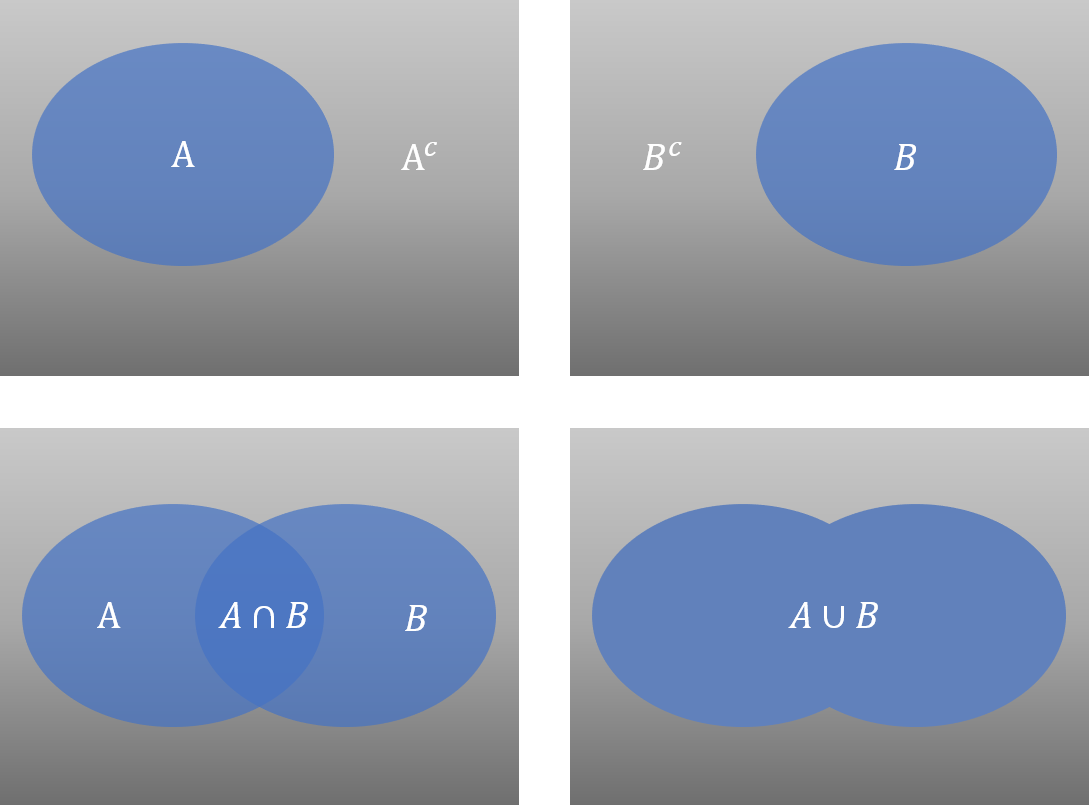
\includegraphics[width=1.0\linewidth]{boolean_algebra.png}
\end{figure}

举个简单的例子,如果$A$表示会打乒乓球的人,$B$表示会打篮球的人;则$A\cap B$表示既会打乒乓球又(AND)会打篮球的人;$A\cup B$表示所有会打乒乓球或者(OR)会打篮球的人;$A^c$表示所有所有不(NOT)会打乒乓球的人。

正如上面例中介绍到的,逻辑连接词$AND$、$OR$和$NOT$描述了由交集、并集和补集操作引起的集合的解释,表明\emph{集合操作(Set Operations)}和\emph{逻辑操作(Logic Operations)}之间存在密切的联系。

当我们能够将代数语句转化为逻辑语句后,我们就可以很容易地定义表示相同逻辑的不同代数。也就是用一个含有一系列用逻辑函数($AND,OR,NOT$)联系起来的变量($a,b,c,\dots$)的数学函数来表示一个或真或假的\emph{逻辑命题(Logical Proposition)}。
表\ref{tb:de_morgan_law}列出了部分所谓的\emph{De-Morgan定律(De-Morgan's Laws)},它给出了基本逻辑命题的句法等效版本。通过使用这些定律,我们可以从$\wedge$的所有实例或$\vee$的所有实例的任何逻辑表达式中系统地消除。这意味着我们可以将非常复杂的逻辑命题简化为形成两种标准形式之一,即连词的分离(即\emph{析取范式,Disjunctive Normal Form})或析取连词(即\emph{连词范式,Conjunctive Normal Form})。

因此,如果我们可以创建一些非常简单的基本门的硬件实现,例如,$NOT$, $AND$和$OR$,我们原则上可以将这些操作组合成非常复杂的电路。在经典的数字电路研究中包括许多这样的模块,比如加法器\cite[]{Mukherjee_Dhar_2014}、乘法器\cite[]{Shu_Haruo_2016}、滤波器\cite[]{Kumar_Agarwal_2021}等等,具体的相关内容将在后续章节进行介绍。

传统上,\emph{逻辑门(Logic Gate, LG)}被认为是一种接受一个或多个布尔值(即$FALSE$或$TRUE$)作为输入,并返回一个布尔值作为输出的物理设备。布尔值($FALSE$和$TRUE$)通常分别与位值$0$和$1$同义使用。逻辑门是现代计算机的关键部件。任何经典计算都可以分解成一系列逻辑门,每次只作用于几个比特。因此,逻辑门是所有现代计算机的核心。整体上各类基本的门电路可以分为两类:\emph{可逆门(Reversible Gate)}和\emph{不可逆门(Irreversible Gate)}。下面两小节将分别介绍他们。

\begin{table}
    \centering
    \caption[De-Morgan定律]{逻辑上等价的命题。这里通过使用\emph{De-Morgan定律},任何命题都可以单独使用$NOT$和$AND$表示,或者单独使用$NOT$和$OR$}
    \label{tb:de_morgan_law}
    \begin{tabular}[\linewidth]{L{8cm}L{4cm}}
        \toprule
        % % \rule{width}{height}
        % \rule{0pt}{1cm} %改变行高
        % \renewcommand\arraystretch{2}  % 2表示2倍行高,个人经验1.2比较好
        \textbf{逻辑等效形式} & \\
        \toprule 
        $a\wedge0=0$ & 0与\\
        $a\wedge1=a$ & 1与\\
        $a\vee 0=1$ & 0或\\
        $a\vee 1=a$ & 1或\\
        \midrule 
        $a\wedge a=a$ & 独立性\\
        $a\vee a=a$ & 独立性\\
        $a\wedge \neg a=0$ & 矛盾定理\\
        $a\vee \neg a=1$ & 无谓重复\\
        $ \neg \neg a=1$ & 双重否定\\
        \midrule 
        $a\vee b=b\vee a$ & 与的交换律\\
        $a\wedge b=b\wedge a$ & 或的交换律\\
        $a\vee (b\vee c)=(a\vee b)\vee c$ & 与的结合律\\
        $a\wedge (b\wedge c)=(a\wedge b)\wedge c$ & 或的结合律\\
        $a\wedge (b\vee c)=(a\wedge b)\vee (a\wedge c)$ & 分配律\\
        $a\vee (b\wedge c)=(a\vee b)\wedge (a\vee c)$ & 分配律\\
        \midrule
        $a\wedge (a\vee b)=a$ & 吸收律\\
        $a\vee (a\vee b)=a$ & 吸收律\\
        $a\wedge (\neg a\vee b)=a\vee b$ & 吸收律\\
        $a\vee (\neg a\vee b)=a\wedge b$ & 吸收律\\
        \midrule
        $\neg(a\wedge b)=(\neg a)\vee (\neg b)$ & De-Morgan定律\\
        $\neg(a\vee b)=(\neg a)\wedge (\neg b)$ & De-Morgan定律\\
        $(a\wedge b)\vee(a\wedge \neg b)=a$ & \\
        $a\Longrightarrow b=\neg a \vee b$ & \\
        $a\Longrightarrow b=\neg (a \vee \neg b)$ & \\
        \bottomrule
    \end{tabular}
\end{table}





\subsubsection[不可逆门:AND、OR、XOR]{不可逆门:AND、OR、XOR}

\begin{figure}
    \centering
    \caption[不可逻辑逆门]{不可逻辑逆门}
    \label{fig:irreversible_gates}
    \subcaptionbox{$AND$门图标\label{fig:and_gate}}{
        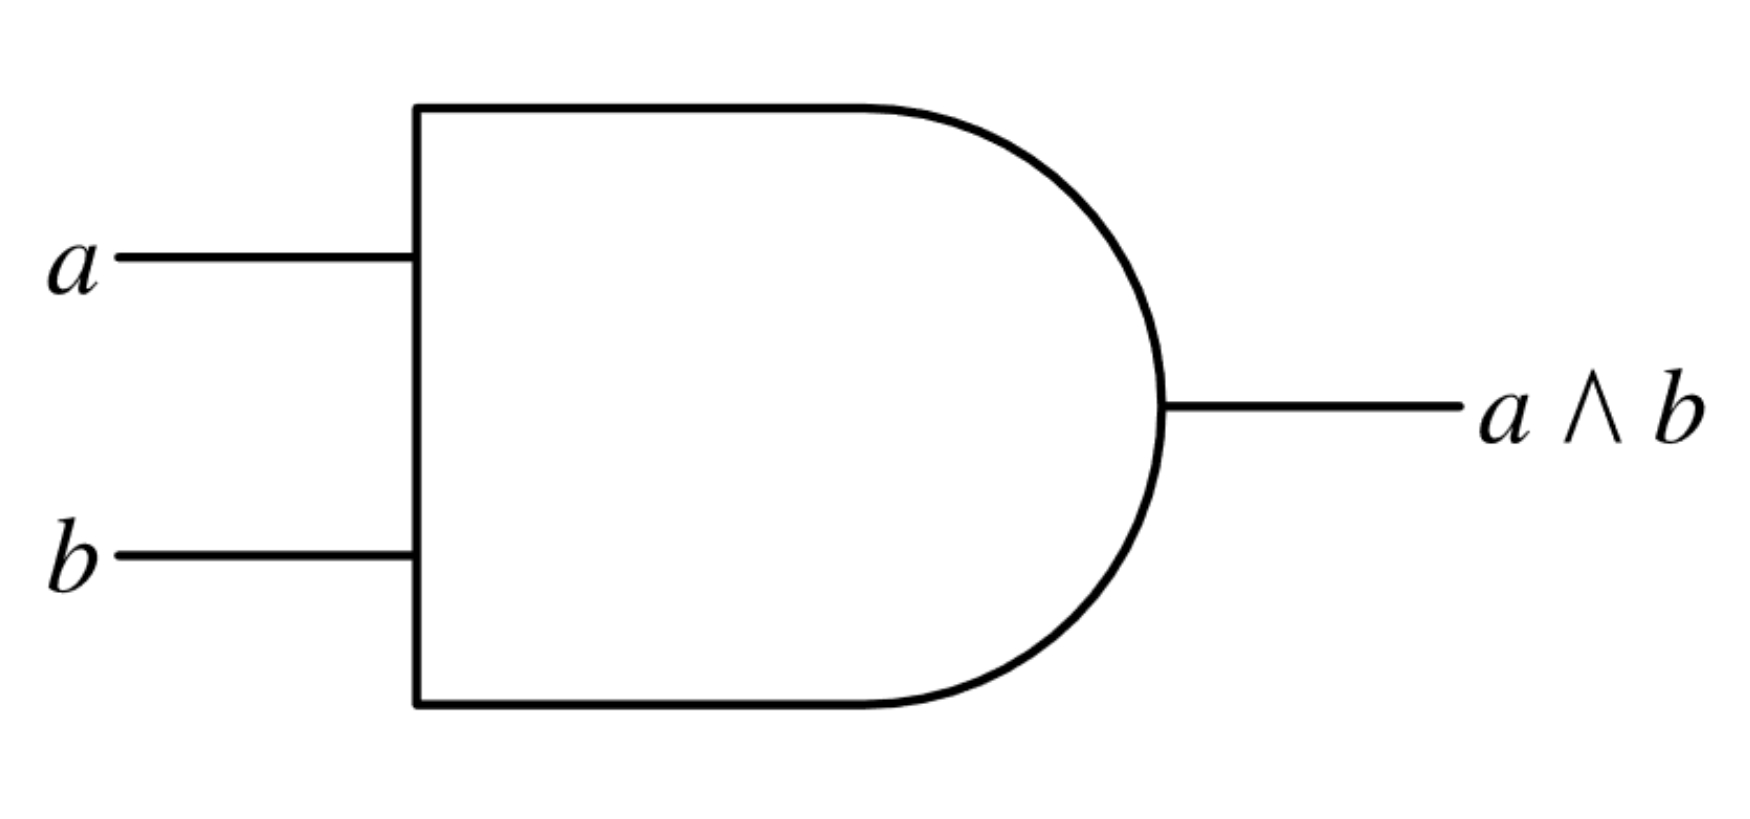
\includegraphics[width=0.3\linewidth]{and_gate.png}
    }
    \subcaptionbox{$OR$门图标\label{fig:or_gate}}{
        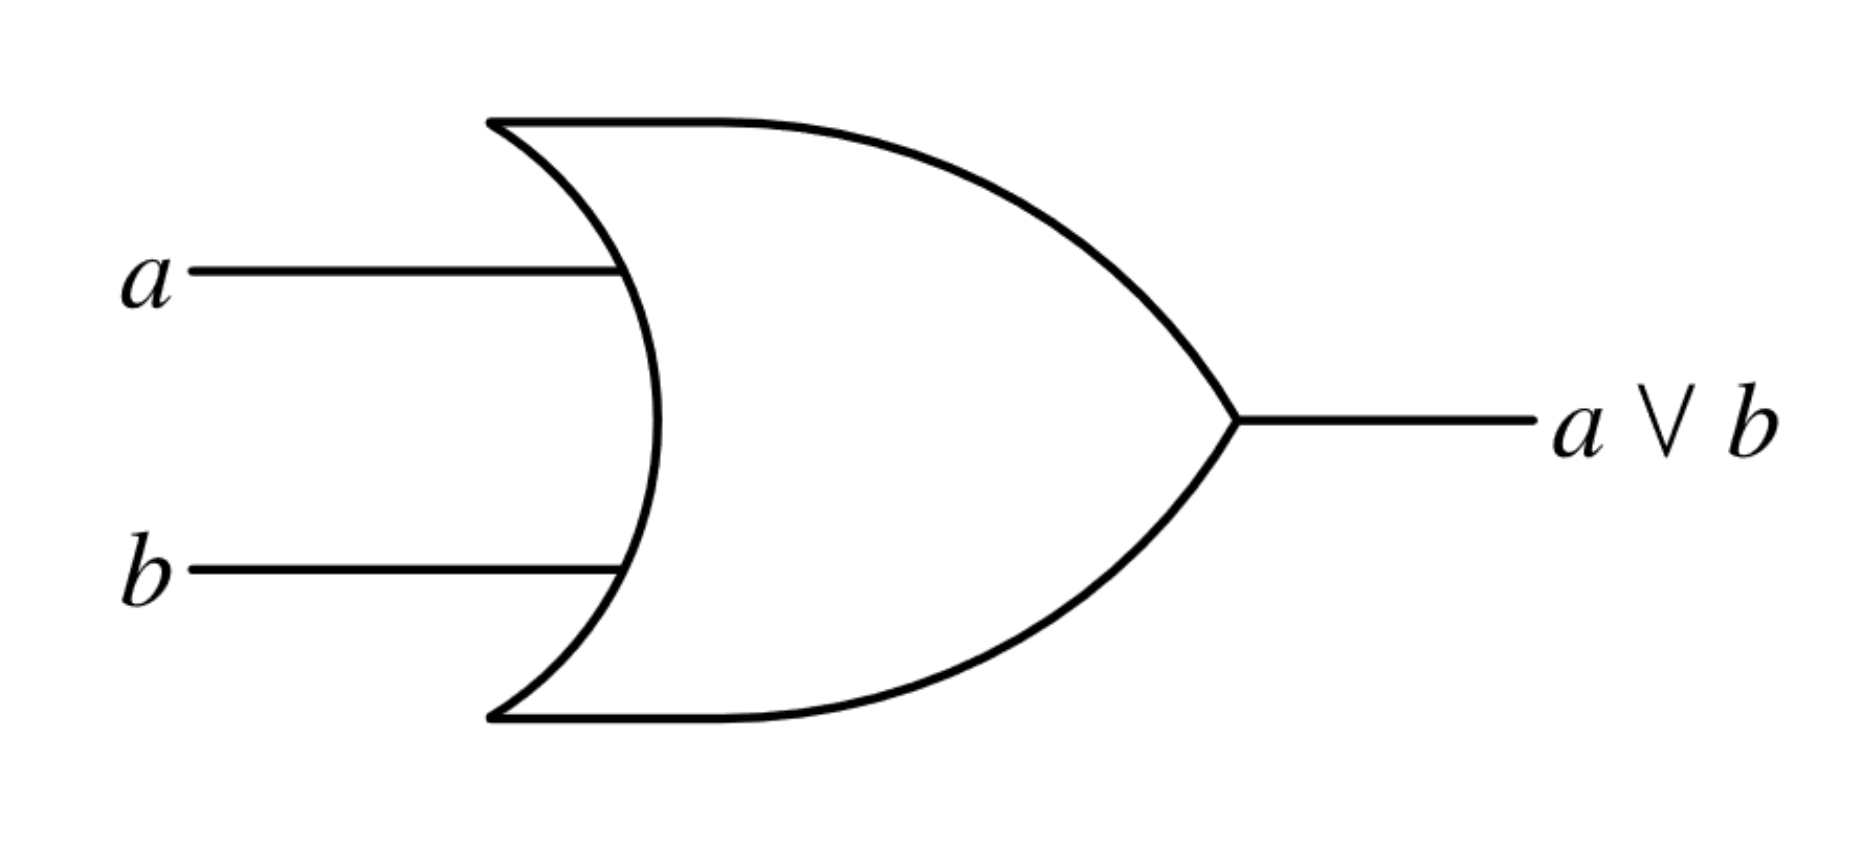
\includegraphics[width=0.3\linewidth]{or_gate.png}
    }
    \subcaptionbox{$XOR$门图标\label{fig:xor_gate}}{
        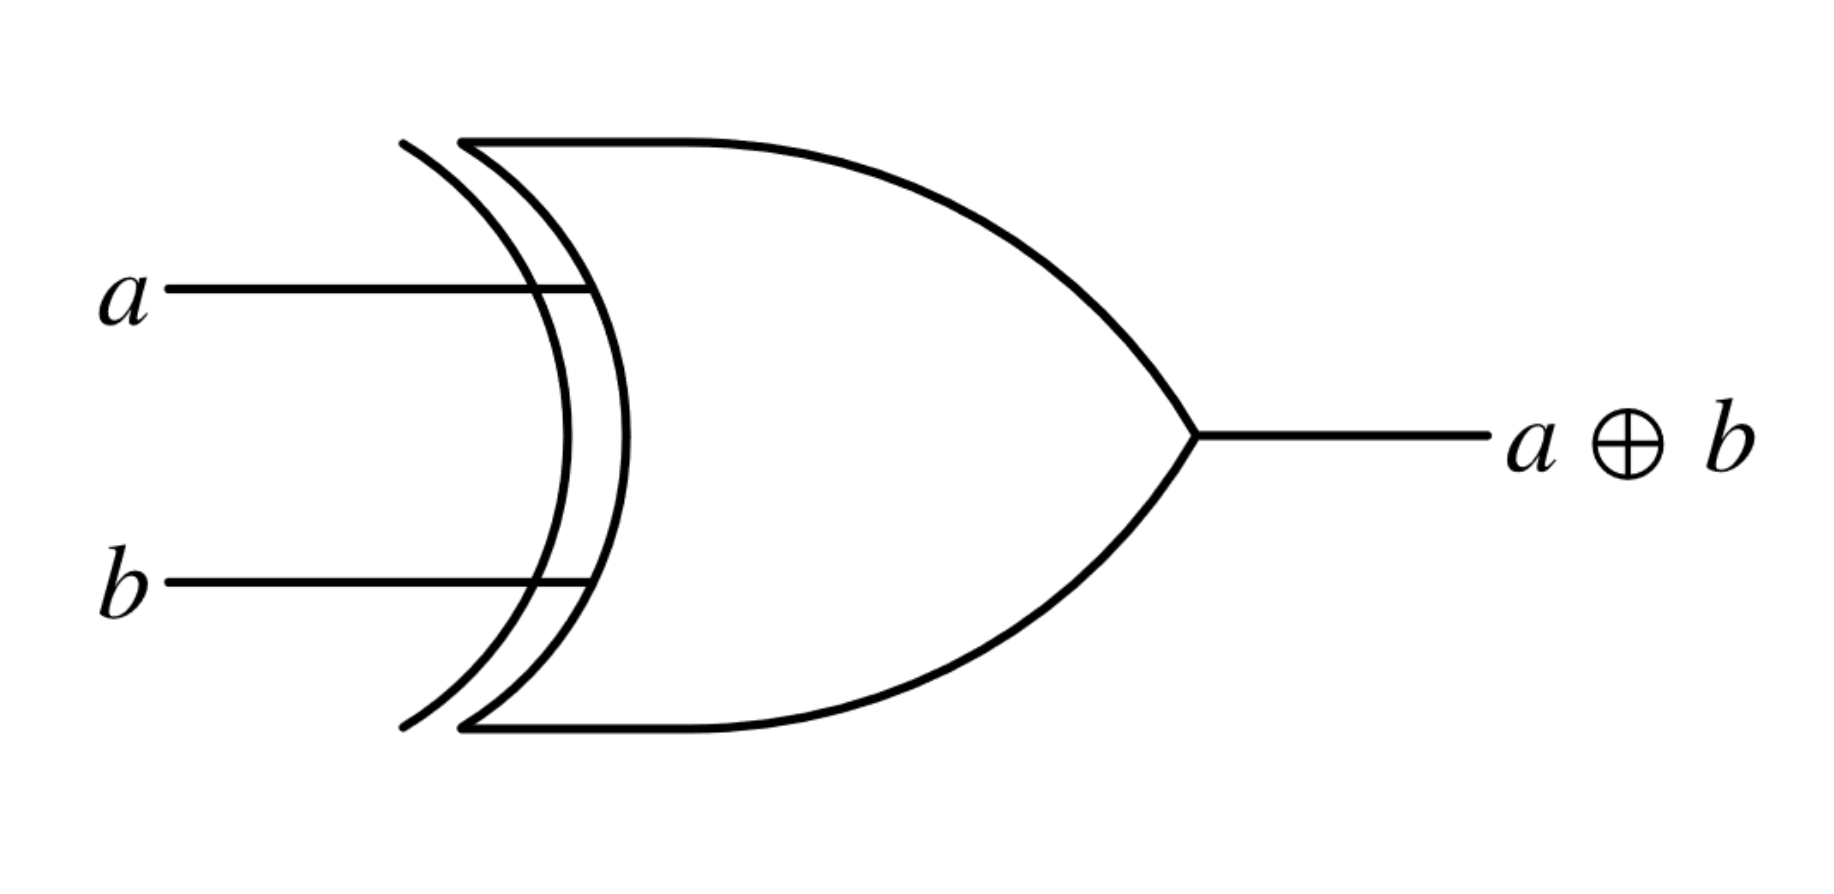
\includegraphics[width=0.3\linewidth]{xor_gate.png}
    }
\end{figure}

\begin{table}
    \centering
    \caption[不可逻辑逆门]{不可逻辑逆门}
    \subcaptionbox{$AND$门真值表\label{tb:and_gate}}{
        \begin{tabular}{C{1cm}C{1cm}C{1cm}}
            \toprule 
            \multicolumn{3}{c}{\textbf{AND}}\\
            \toprule
            a & b & $a\wedge b$ \\
            \hline
            0 & 0 & 0\\
            0 & 1 & 0\\
            1 & 0 & 0\\
            1 & 1 & 1\\
            \bottomrule
        \end{tabular}
    }
    \subcaptionbox{$OR$门的真值表\label{tb:or_gate}}{
        \begin{tabular}{C{1cm}C{1cm}C{1cm}}
            \toprule 
            \multicolumn{3}{c}{\textbf{OR}}\\
            \toprule
            a & b & $a\vee b$ \\
            \hline
            0 & 0 & 0\\
            0 & 1 & 1\\
            1 & 0 & 1\\
            1 & 1 & 1\\
            \bottomrule
        \end{tabular}
    }
    \subcaptionbox{$XOR$门的真值表\label{tb:xor_gate}}{
        \begin{tabular}{C{1cm}C{1cm}C{1cm}}
            \toprule 
            \multicolumn{3}{c}{\textbf{XOR}}\\
            \toprule
            a & b & $a\bigoplus b$ \\
            \hline
            0 & 0 & 0\\
            0 & 1 & 1\\
            1 & 0 & 1\\
            1 & 1 & 0\\
            \bottomrule
        \end{tabular}
    }
    
\end{table}


描述逻辑门动作的最好方法是用它的\emph{真值表(Truth Table)}。在真值表中,我们写下输入的所有可能的逻辑值及其相应的输出。例如,$AND$门的真值表如表\ref{tb:and_gate}所示。$AND$门在电路图中对应的图标如图\ref{fig:and_gate}所示。$AND$门在逻辑上是不可逆的,属于\emph{不可逆逻辑门(Irreversible Logic Gate, ILG)},这意味着我们无法为所有输出确定唯一的输入。具体来说,如果输出为$0$(即$FALSE$),则无法判断输入值是$00$、$01$还是$10$。换句话说,当$AND$门的输出为$0$时,它就会“擦除”一些信息。

同理,$OR$门的真值表如表\ref{tb:or_gate}所示。$OR$门对应的电路图标如图\ref{fig:or_gate}所示。$OR$门在逻辑上也是不可逆的,因为当它的输出为$1$(即$TRUE$)时,不可能说输入是$01$、$10$还是$11$。也就是说,当输出为$1$时,$OR$门再次擦除一些信息。

$OR$门有一种很常见变体,称为\emph{异或门(Exclusive-OR Gate)}(通常写为$XOR$或$\bigoplus$),事实证明它非常有用(因为很容易用晶体管实现)。$XOR$与$OR$相似,不同之处在于当两个输入都为$1$(即$TRUE$)时,它返回$0$(即$FALSE$)。$XOR$的真值表如表\ref{tb:xor_gate}所示。相应的异或电路图标如图\ref{fig:xor_gate}所示。




\subsubsection[可逆逻辑门:NOT、SWAP、CNOT]{可逆逻辑门:NOT、SWAP、CNOT}

上节介绍到的如$AND$门、$OR$门、$XOR$门等不可逆门在实践中应用十分广泛。随着数字芯片技术的不断发展,由于集成化的散热问题,不可逆门天然存在的限制逐渐被人们关注。基础物理理论告诉我们当信息被擦除时,一定伴随着能量的耗散\cite[]{Kastner_Schlatter_2023}。具体来说,每一比特信息的擦除会释放的能量为$kT\ln 2$,其中$k$是玻尔兹曼常数($k=1.3805\times 10^{-23}JK^{-1}$)而$T$是以\emph{凯尔文(Kelvin)}为单位的绝对温度。因此,即使所有其它能量损失机制从电路中消除了,由于信息擦除时发生的不可避免的能量损失,电路在操作时仍然会耗散能量。尽管当今在逻辑电路中由于逻辑不可逆性而导致的这种能量耗散与其它机制导致的能量耗散相比还比较小。然而,随着其它机制导致的能量耗散不断被克服,这种不可避免的信息擦除能量耗散将成为重要贡献,这将会阻碍计算芯片的进一步小型化和集成化。

克服上述问题的其中一个解决方案是修改现有的逻辑门使其仅使用\emph{可逆逻辑门(Reversible Logic Gate, RLG)}实现。在可逆逻辑门中,一个输入对应着一个确定的输出,反之亦然。因此,可逆门在起作用时永远不会删除任何信息,因此,可以向前运行基于可逆逻辑的计算以获得答案、复制的答案以及整个计算,然后再反向执行整个过程以恢复除用于复制中间点答案的小部分能量之外的所有能量。

可逆逻辑门的最简单例子是$NOT$门。$NOT$是一个\emph{1-input/1-output}门,它简单地反转它所处理的位值。$NOT$门的真值表如表\ref{tb:not_gate}所示。$NOT$门的电路图标如图\ref{fig:not_gate}所示。如果一个人知道输出位值,就可以明确地推断输入位值,反之亦然。

量子计算中非常重要的可逆门是\emph{受控非门($CNOT$)}。$CNOT$的真值表如表\ref{tb:cnot_gate}所示。$CNOT$门的电路图标如图2.9所示。$CNOT$门的效果是当且仅当第一个位设置为$1$时翻转第二个位的位值。也就是说,否定或不否定第二个位的决定由第一个位的值控制。这也是叫它受控非门的原因。
\begin{figure}
    \centering
    \caption{$NOT$门图标\label{fig:not_gate}}
    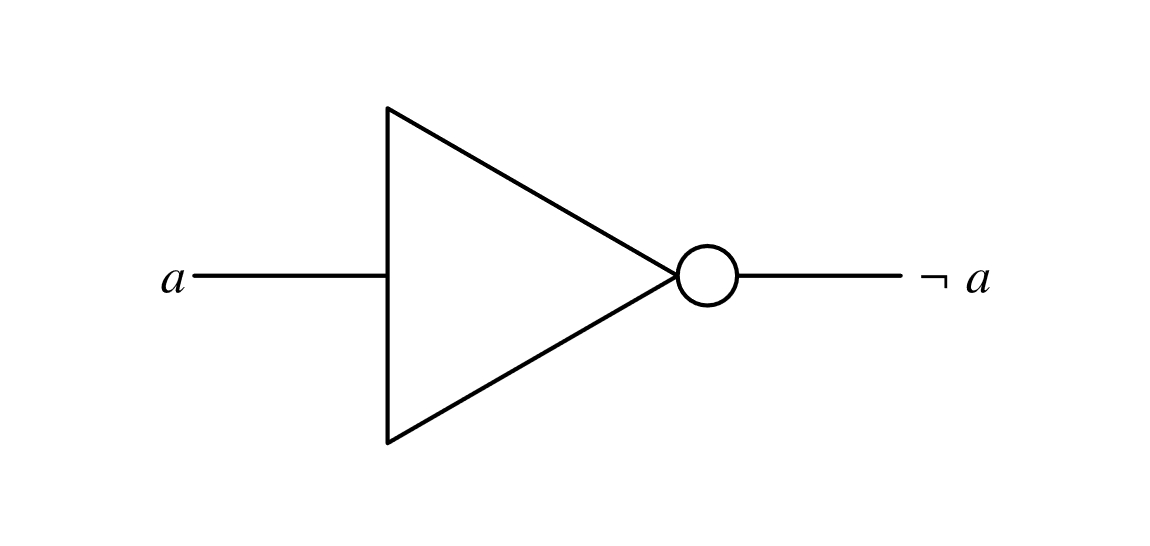
\includegraphics[width=0.8\linewidth]{not_gate.png}
\end{figure}

\begin{table}
    \centering
    \caption[\emph{NOT}门]{\emph{NOT}门\label{tb:not_gate}}
    \begin{tabular}{C{1.5cm}C{1.5cm}}
        \toprule 
        \multicolumn{2}{c}{\textbf{NOT}}\\
        \toprule
        a & $\neg a$  \\
        \hline
        0 & 1 \\
        1 & 0 \\
        \bottomrule
    \end{tabular}
\end{table}


\begin{figure}
    \centering
    \caption{$CNOT$门图标\label{fig:cnot_gate}}
    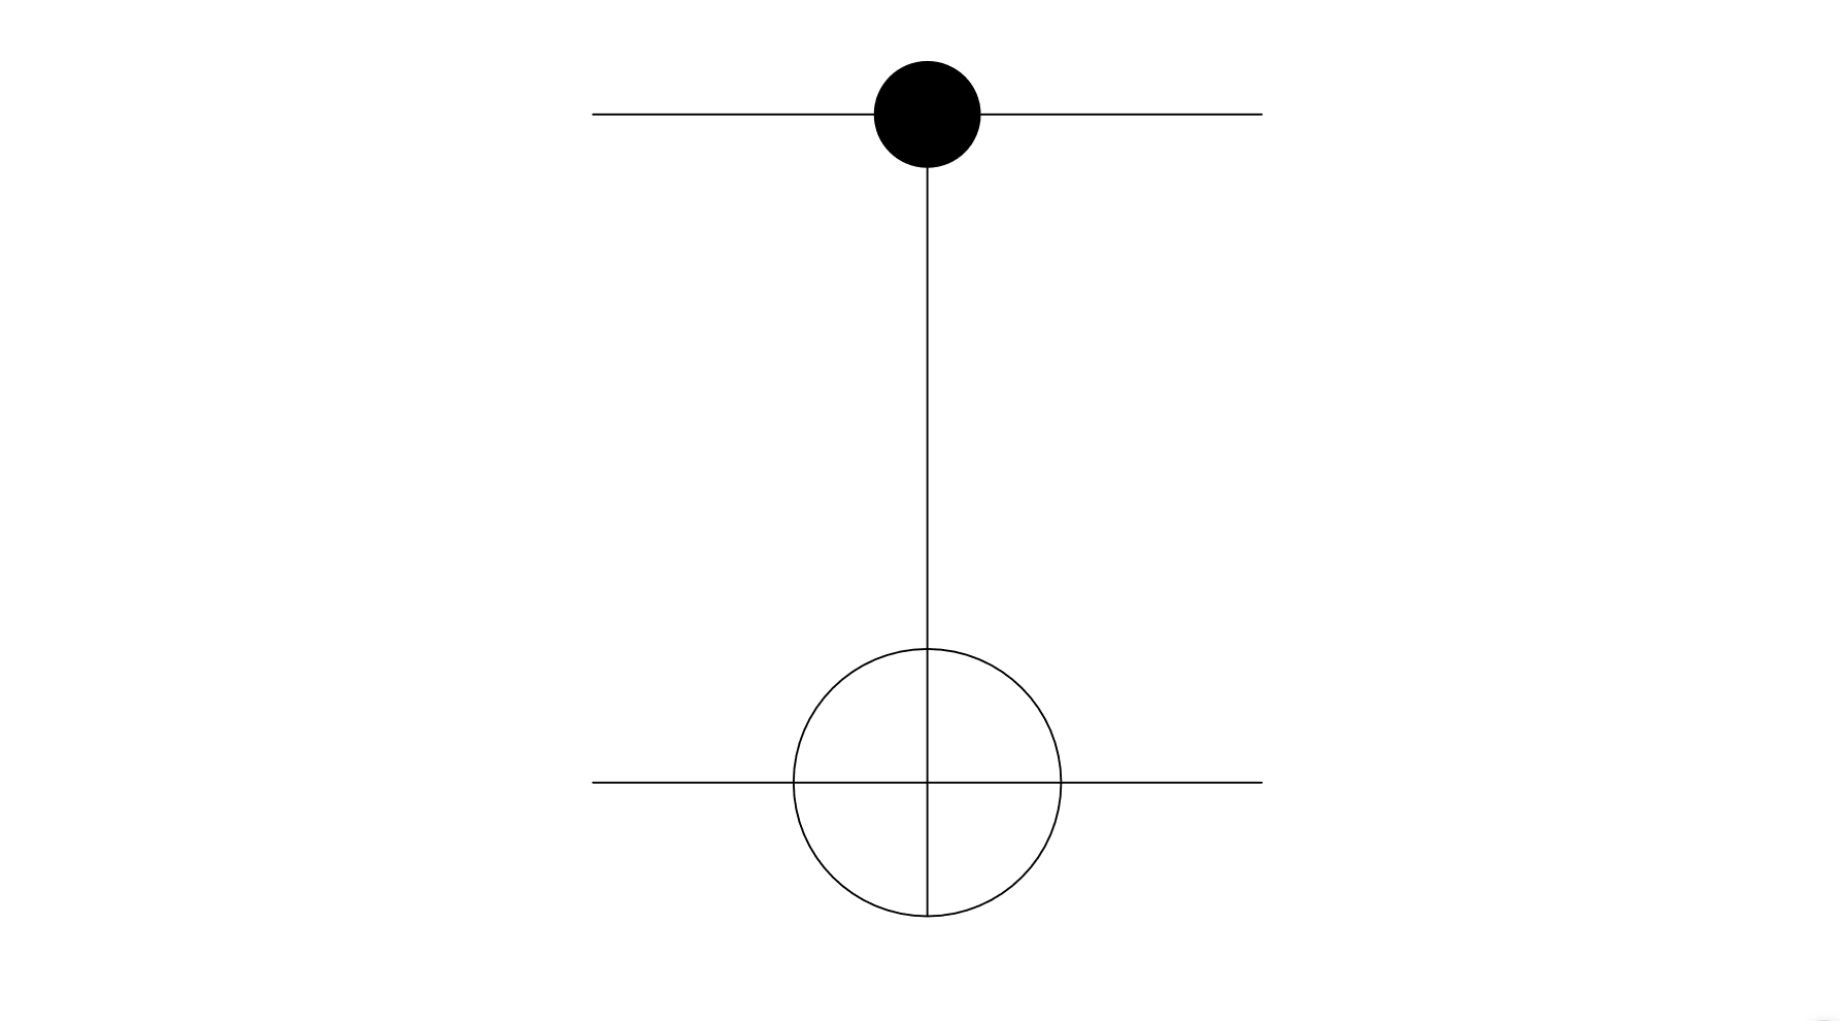
\includegraphics[width=0.8\linewidth]{cnot_gate.png}
\end{figure}

\begin{table}
    \centering
    \caption[\emph{CNOT}门]{\emph{CNOT}门\label{tb:cnot_gate}}
    \begin{tabular}{C{1cm}C{1cm}C{1cm}C{1cm}}
        \toprule 
        \multicolumn{4}{c}{\textbf{CNOT}}\\
        \toprule
        a & b & $a'$ & $b'$  \\
        \hline
        0 & 0 & 0 & 0 \\
        0 & 1 & 1 & 0 \\
        1 & 0 & 0 & 1 \\
        1 & 1 & 1 & 1 \\
        \bottomrule
    \end{tabular}
\end{table}
% \begin{figure}
%     \centering
%     \caption[可逆逻辑门]{可逆逻辑门}
%     \label{fig:reversible_gates}
%     \subcaptionbox{$NOT$门图标\label{fig:not_gate}}{
%         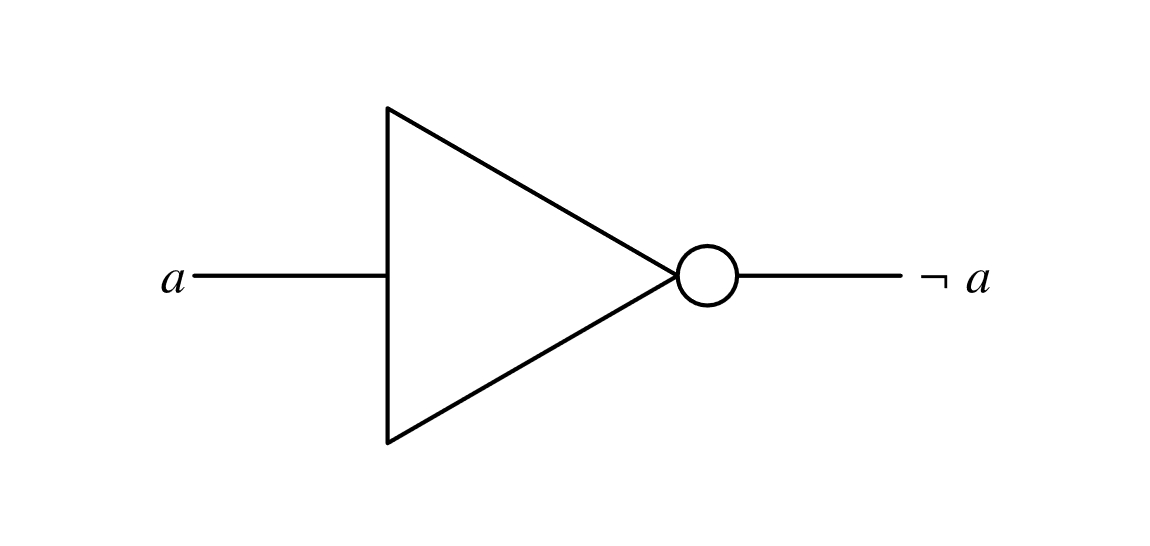
\includegraphics[width=0.45\linewidth]{not_gate.png}
%     }
%     \subcaptionbox{$CNOT$门图标\label{fig:cnot_gate}}{
%         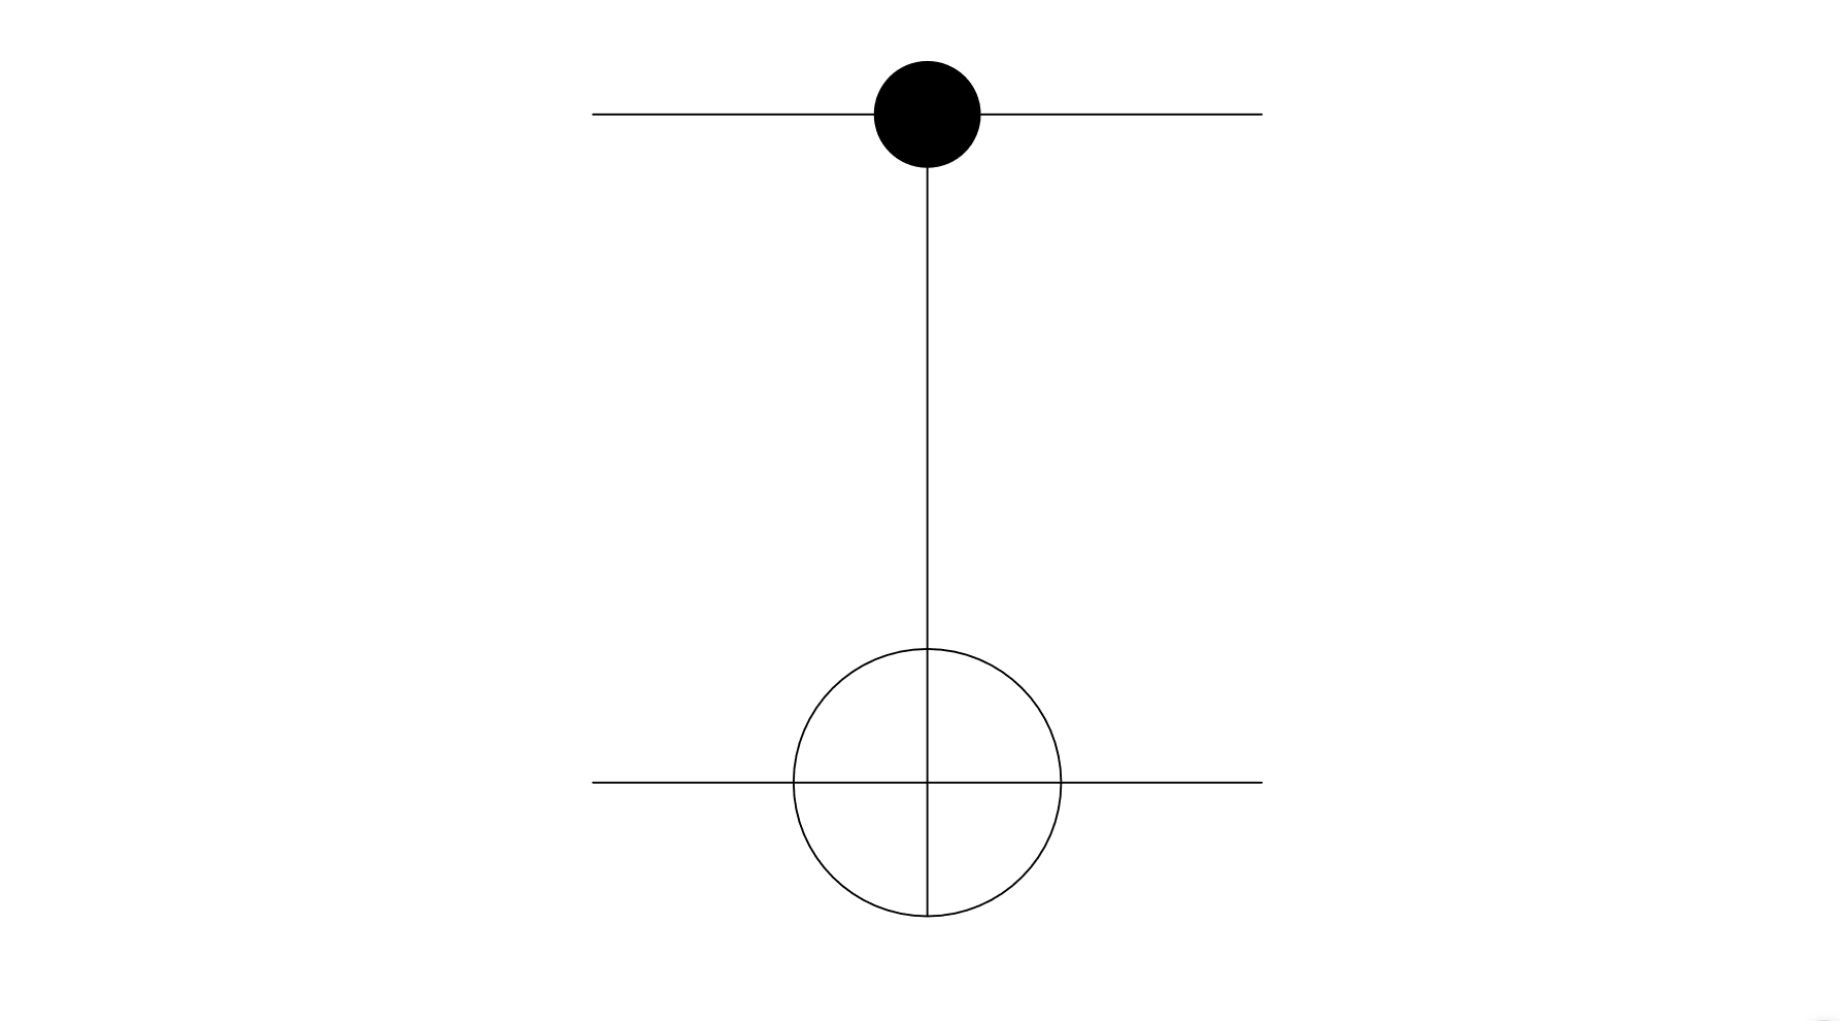
\includegraphics[width=0.45\linewidth]{cnot_gate.png}
%     }
% \end{figure}

% \begin{table}
%     \centering
%     \caption[可逆逻辑门]{可逆逻辑门}
%     \subcaptionbox{\emph{NOT}门\label{tb:not_gate}}{
%         \begin{tabular}{C{1.5cm}C{1.5cm}}
%             \toprule 
%             \multicolumn{2}{c}{\textbf{NOT}}\\
%             \toprule
%             a & $\neg a$  \\
%             \hline
%             0 & 1 \\
%             1 & 0 \\
%             \bottomrule
%         \end{tabular}
%     }
%     \subcaptionbox{\emph{CNOT}门\label{tb:cnot_gate}}{
%         \begin{tabular}{C{1cm}C{1cm}C{1cm}C{1cm}}
%             \toprule 
%             \multicolumn{4}{c}{\textbf{CNOT}}\\
%             \toprule
%             a & b & $a'$ & $b'$  \\
%             \hline
%             0 & 0 & 0 & 0 \\
%             0 & 1 & 1 & 0 \\
%             1 & 0 & 0 & 1 \\
%             1 & 1 & 1 & 1 \\
%             \bottomrule
%         \end{tabular}
%     }
% \end{table}




注意$CNOT$门不仅是一种RLG,还是一种\emph{通用逻辑门(Universal Logic Gate, ULG)}。也就是说以它为基础可以实现任何其它类型的门,比如$AND$、$OR$等等,进一步地可以只用$CNOT$搭建网络实现任何计算。ULG除了$CNOT$门外,还有$TOFFOLI$门\cite[]{Maslov_Dueck_Miller_2005}、$FREDKIN$门\cite[]{Adamatzky_2017}等等。$TOFFOLI$门和$FREDKIN$门都属于RLG,比如$TOFFOLI$门的真值表如表\ref{tb:toffoli_gate}所示,它的图标如图\ref{fig:toffoli_gate}所示。
\begin{table}
    \centering
    \caption[TOFFOLI]{\emph{TOFFOLI}门真值表}
    \label{tb:toffoli_gate}
    \begin{tabular}{C{1cm}C{1cm}C{1cm}C{1cm}C{1cm}C{1cm}}
        \toprule
        a & b & c & $a'$ & $b'$ & $c'$\\
        \toprule 
        0 & 0 & 0 & 0 & 0 & 0\\
        0 & 0 & 1 & 0 & 0 & 1\\
        0 & 1 & 0 & 0 & 1 & 0\\
        0 & 1 & 1 & 0 & 1 & 1\\
        1 & 0 & 0 & 1 & 0 & 0\\
        1 & 0 & 1 & 1 & 0 & 1\\
        1 & 1 & 0 & 1 & 1 & 1\\
        1 & 1 & 1 & 1 & 1 & 0\\
        \bottomrule
    \end{tabular}
\end{table}
\begin{figure}
    \centering
    \caption[\emph{TOFFOLI}门图标]{\emph{TOFFOLI}门图标}
    \label{fig:toffoli_gate}
    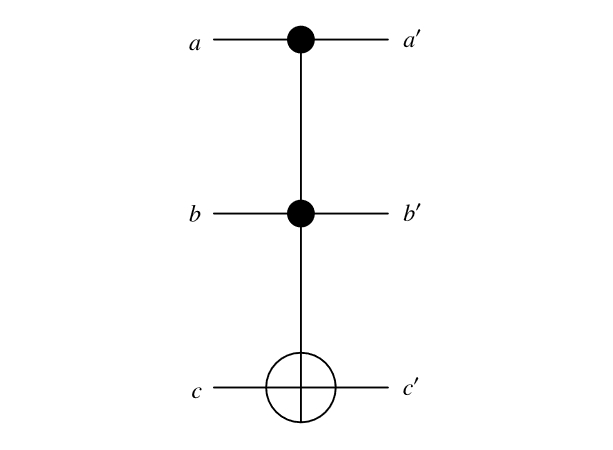
\includegraphics[width=0.8\linewidth]{toffoli_gate.png}
\end{figure}

\subsection[量子逻辑门]{量子逻辑门}
前面我们已经讨论过经典的不可逆和经典的可逆门,这使我们能够更好地理解量子门的优越性。就像任何经典计算都可以分解成一系列经典逻辑门,这些门一次只作用于几个经典比特,因此任何量子计算也可以分解成一系列量子逻辑门,这些门一次只作用于几个量子比特。主要区别在于,虽然经典逻辑门操纵经典位值$0$或$1$,但量子门可以操纵任意多量子态,包括计算基态的任意叠加,这些量子态也经常纠缠在一起。因此,量子计算的逻辑门比经典计算的逻辑门更加多样化。

通常我们使用\emph{泡利矩阵(Pauli Matrices)},$\mathbb{1}, \mathbfit{X}, \mathbfit{Y}, \mathbfit{Z}$,来描述单量子比特。单量子比特既是厄米特(Hermitian)的也是幺正(Unitary)的,任何1-量子比特哈密顿量总是可以写成泡利矩阵的加权和:
\begin{align}
    \mathbb{1}=\begin{pmatrix}
        1 & 0 \\
        0 & 1 \\
    \end{pmatrix}, \quad \mathbfit{X}=\begin{pmatrix}
        0 & 1 \\
        1 & 0 \\
    \end{pmatrix}, \quad  \mathbfit{Y}=\begin{pmatrix}
        0 & -i \\
        i & 0 \\
    \end{pmatrix}, \quad  \mathbfit{Z}=\begin{pmatrix}
        1 & 0 \\
        0 & -1 \\
    \end{pmatrix}
\end{align}

实际上泡利矩阵$\mathbfit{X}$和经典逻辑门中的$NOT$门对应,有:
\begin{align}
    \mathbfit{X}\equiv NOT = \begin{pmatrix}
        0 & 1 \\
        1 & 0 \\
    \end{pmatrix}
\end{align}

也就是说$\mathbfit{X}$可以类似经典比特的$NOT$门用来翻转量子比特的状态,即:
\begin{align}
    \mathbfit{X}\ket{0}=\begin{pmatrix}
        0 & 1 \\
        1 & 0 \\
    \end{pmatrix}\cdot \begin{pmatrix}
         1 \\
         0 \\
    \end{pmatrix}=\begin{pmatrix}
        0 \\
        1 \\
   \end{pmatrix}=\ket{1}\\
   \mathbfit{X}\ket{1}=\begin{pmatrix}
    0 & 1 \\
    1 & 0 \\
\end{pmatrix}\cdot \begin{pmatrix}
     0 \\
     1 \\
\end{pmatrix}=\begin{pmatrix}
    1 \\
    0 \\
\end{pmatrix}=\ket{0}\\
\end{align}

但是注意$\mathbfit{X}$并不是一个真正意义上的\emph{量子非门(Quantum Not Gate, QNG)},实际上并不存在一个通用的QNG。

有一个很重要的量子门值得在这里被介绍,它就是\emph{Hadamard门(Hadamard Gate)},它的定义如下\cite[]{PRUDÊNCIO_2013}:
\begin{align}
    \mathbfit{H}=\frac{1}{\sqrt{2}}\begin{pmatrix}
        1 & 1 \\
        1 & -1 \\
    \end{pmatrix}
\end{align}

它的最广泛的应用是用来制备量子叠加态,基本的过程示意如下:
\begin{align}
    \mathbfit{H}\ket{0}=\frac{1}{\sqrt{2}}\begin{pmatrix}
        \ket{0}+\ket{1}
    \end{pmatrix}\\
    \mathbfit{H}\ket{1}=\frac{1}{\sqrt{2}}\begin{pmatrix}
        \ket{0}-\ket{1}
    \end{pmatrix}\\
\end{align}

这是一个看似简单的看门,但它有一个重要的性质。进一步地,它可以制备$n$个比特的叠加态,这些态将会均匀地分布在$[0, 1, ..., 2^n-1]$的范围上:
\begin{align}
    \mathbfit{H}\ket{0}\otimes\mathbfit{H}\ket{0}\otimes\dots\otimes\mathbfit{H}\ket{0}=\frac{1}{\sqrt{2^n}}\sum_{j=0}^{2^n-1}\ket{j}
\end{align}

其中$\ket{j}$是是由二进制数索引的计算基态,该二进制数将对应于 十进制符号中的数字$j$。比如对于$3$量子比特的寄存器来说,$\ket{0}$表示计算基态$\ket{000}$;$\ket{1}$表示计算基态$\ket{001}$;··· ;$\ket{7}$表示计算基态$\ket{111}$。

这些本征态意味着可以使用$n$比特同时写入的所有可能比特串组合。它实际上是量子计算最重要的技巧之一,因为它实现了仅使用多项式多次操作而将指数多的索引加载到量子计算机中。如果自然界没有种方法,我们则必须像我们在经典计算中所做的那样一个一个单独输入不同的位串,那么量子计算在计算复杂性方面取得突破的可能性要小得多。

在量子门的阐述中有一个门是绝对不能忽略的,那就是量子$CNOT$门。和经典$CNOT$门一样,它会根据一个比特的状态来决定是否翻转两一个比特的状态,比如:
\begin{align}
    \ket{00}\overset{CNOT}{\longrightarrow}\ket{00}\\
    \ket{01}\overset{CNOT}{\longrightarrow}\ket{01}\\
    \ket{10}\overset{CNOT}{\longrightarrow}\ket{11}\\
    \ket{11}\overset{CNOT}{\longrightarrow}\ket{10}\\
\end{align}

其中第二个比特(靠右的)的状态受到第一个比特(靠左的)的状态控制。由于$CNOT$门是一个通用的门,因此只要一个量子物理体系能够实现$CNOT$门,那么这个体系就具备了实现通用量子计算机的前景\cite[]{Zajac_Sigillito_Russ_Borjans_Taylor_Burkard_Petta_2018,Zhu_Cheng_Zhu_Chen_Guan_2022}。


\subsection[量子算法]{量子算法}









\section[量子计算的不同实现平台]{量子计算的不同实现平台}
\textcolor{red}{这部分需要分别找各个平台的文献进行整理,每个平台找一到两篇吧}
\subsection[离子量子计算]{离子量子计算}

\subsection[超导量子计算]{超导量子计算}

\subsection[原子量子计算]{原子量子计算}

\subsection[硅基量子计算]{硅基量子计算}

\subsection[光量子计算]{光量子计算}

\subsection[拓扑量子计算]{拓扑量子计算}







% !TeX root = ../sustechthesis-example.tex

\chapter[离子阱量子计算系统]{离子阱量子计算系统\label{section:ion_trap_quantum_computation_system}}

% \textcolor{red}{
% 这部分简单讲一下离子阱量子计算的发展历史,重点介绍离子阱量子计算系统的基本组成,不针对特别具体的系统...
% }

% \section[离子阱的发展]{离子阱的发展}

% \textcolor{red}{这部分主要参考文献\cite[p2]{Bruzewicz_Chiaverini_McConnell_Sage_2019}}




% \section[离子阱的囚禁]{离子阱的囚禁}

\section[离子在RF阱中的经典运动]{离子在RF阱中的经典运动\label{section:ion_classical_motion}}
% \textcolor{red}{主要参考文献\cite[chap2-A]{Leibfried_Blatt_Monroe_Wineland_2003}}

离子阱采用射频阱对离子进行动态囚禁,最具代表性的一类是四极阱,它及它的一些变型也是目前在离子阱量子计算研究中应用最广泛的一类离子阱。四极阱的电势描述如下:
\begin{align}
    % \label{eq:quadrupolar_trap_potential}
    \Phi(x, y, z, t) = &U\frac{1}{2}(\alpha x^2 + \beta y^2 + \gamma z^2) \label{eq:time_independent_part}\\
    \label{eq:time_dependent_part}
    &+ \tilde{U}\cos (\omega_{rf}t)\frac{1}{2}(\alpha ' x^2 + \beta ' y^2 + \gamma ' z^2) 
\end{align}
其中$\Phi(x, y, z, t)$是四极阱的电势,公式\eqref{eq:time_independent_part}是不依赖时间的项,公式\eqref{eq:time_dependent_part}是随时间变化的项。整个电势的表达式每时每刻都要满足拉普拉斯方程(Laplace equation)$\Delta \Phi=0$的约束条件,从中可以导出整个四极阱的几何参数约束:
\begin{align}
    \alpha + \beta + \gamma =0,\\
    \alpha ' + \beta ' + \gamma ' =0
\end{align}

其中各参数的定义在公式\eqref{eq:time_independent_part}和公式\eqref{eq:time_dependent_part}定义。从这些限制可以明显看出,在自由空间中电势不可能稳定地产生局部三维最小值,因此电势只可能以动态方式来对离子进行囚禁。幸运的是,通过对四极阱几何参数的选择,再结合适当的驱动微波的频率和驱动电压我们可以做到这一点。其中一种几何参数选择如下:
\begin{align}
    -(\alpha + \beta )= \gamma > 0,\\
    \alpha ' = - \beta '
\end{align}
这种几何参数的设置会使离子在$x,y$平面上动态地被囚禁,在$z$方向上静态地被囚禁。在这种设置的离子阱中,多个离子会沿着$z$轴形成线性的离子链,这便是人们所知的\emph{线性离子阱(Linear Trap)},也被称为\emph{Paul Trap}\cite[]{Paul_1990}。在接下来的两小节里我将介绍囚禁离子的经典运动方程及其解析解(第\ref{section:classical_motion}节),并给出这些解的低阶近似(第\ref{section:lowest_order_approximation}节)。

\subsection[经典运动方程]{经典运动方程\label{section:classical_motion}}

一个质量为$m$电荷量为$Z|e|$的粒子在如公式\eqref{eq:time_independent_part}所描述的电场中的经典运动方程由Paul等人\cite[p415]{Paul1958}给出。粒子的运动在空间坐标方向上中是解耦的。下面只讨论$x$方向上的运动;其他方向可以类似地处理。运动方程如下:
\begin{align}
    \ddot{x}=-\frac{Z|e|}{m}\frac{\partial \Phi}{\partial x}=-\frac{Z|e|}{m}[U\alpha + \tilde{U}\cos(\omega_{rf}t)\alpha ']x
\end{align}

经过下面的参数代换,这个方程可以转化为标准的\emph{马修方程(Mathieu Equation, ME)}形式:
\begin{align}
    \frac{d^2x}{d\xi^2}+[a_x-2q_x\cos(2\xi)]x=0\label{eq:mathieu_equation}
\end{align}

相应的参数代换为:
\begin{align}
    \xi=\frac{\omega_{rf}t}{2},\ a_x=\frac{4Z|e|U\alpha}{m\omega_{rf}^2},\ q_x=\frac{2Z|e|\tilde{U}\alpha '}{m\omega_{rf}^2}\label{eq:parameters_substitution}
\end{align}

ME方程属于一般的周期系数微分方程。它的稳定解的一般形式可以由\emph{弗洛奎定理(Floquet Theorem)}导出\cite[]{McLachlan, McQuarrie}:
\begin{align}
    x(\xi)=&Ae^{i\beta_x\xi}\sum_{n=-\infty}^{\infty}C_{2n}e^{i2n\xi}\\
    &+ Be^{-i\beta_x\xi}\sum_{n=-\infty}^{\infty}C_{2n}e^{-i2n\xi}\label{eq:mathieu_solution}
\end{align}

其中实值特征指数$\beta_x$和系数$C_{2n}$仅是$a_x$和$q_x$的函数,不依赖于初始条件。$A$和$B$是任意常数,可用于满足边界条件或规格化特解。将公式\eqref{eq:mathieu_solution}代入公式\eqref{eq:mathieu_equation}可以得到一个递归关系:
\begin{align}
    C_{2n+2}-D_{2n}C_{2n}+C_{2n-2}=0,\\
    D_{2n}=[a_x-(2n+\beta_x)^2]/q_x\label{eq:recursion_raltion}
\end{align}

这一递归关系将实值特征指数$\beta_x$、系数$C_{2n}$与$a_x$、$q_x$联系起来。通过进一步地整理也可以得到$C_{2n}$的表达式:
\begin{align}
    C_{2n+2}=\frac{C_{2n}}{D_{2n}-\frac{1}{D_{2n+2}-\frac{1}{\dots}}}\\
    C_{2n}=\frac{C_{2n-2}}{D_{2n}-\frac{1}{D_{2n-2}-\frac{1}{\dots}}}\label{eq:c_2n_fraction}
\end{align}

利用结合上述公式$\beta_x$也可以计算:
\begin{align}
    \beta_x^2=a_x-q_x\left(\frac{1}{D_0-\frac{1}{D_2-\frac{1}{\dots}}} + \frac{1}{D_0-\frac{1}{D_{-2}-\frac{1}{\dots}}}\right) \label{eq:beta_x_fraction}
\end{align}

可以根据所需的精度,选择截断公式\eqref{eq:c_2n_fraction}和公式\eqref{eq:beta_x_fraction}中的连分式来获取相应的结果。
实际上,对于实验中常用到的典型$a_x$和$q_x$值,连分式中高阶项的贡献会迅速下降。

% \textcolor{red}{这里的$a_x, q_x$具体的含义后面有时间了可以再看看。}

\subsection[低阶近似]{低阶近似\label{section:lowest_order_approximation}}
实际实验系统中采用的在公式\eqref{eq:parameters_substitution}中定义的参数往往是满足$(|a_x|,q_x^2)\ll 1$的。在此条件下,假设$C_{\pm 4}\simeq 0$,则可以得到$x(t)$轨迹的\emph{低阶近似(Lowest-order Approximation)}。再同时设置初始条件$A=B$,公式\ref{eq:recursion_raltion}可以得到:
\begin{align}
    \beta_x\approx \sqrt{a_x+q_x^2/2},\\
    x(t)\approx2AC_0\cos\left(\beta_x\frac{\omega_{rf}}{2}t\right)\left[1-\frac{q_x}{2}\cos(\omega_{rf}t)\right]\label{eq:classical_motion_solution}
\end{align}

囚禁离子在$x$方向上的轨迹$x(t)$的由频率为$\nu=\beta_x\omega_{rf}/2\ll \omega_{rf}$的谐波振荡叠加频率为$\omega_{rf}$的RF频率造成的\emph{驱动位移}组成,分别称为\emph{长期运动(Secular-motion)}和\emph{微运动(Micro-motion)}两者相位相差$180^\circ$;
离子在离子阱中的微运动的频率为$\omega_{rf}\ll \nu$,且其振幅为长期运动振幅的$q_x/2\ll 1$,这也是它被称为微运动的原因。如果忽略微运动,则长期运动可以近似为频率为$\nu$的谐振子的运动。在大多数情况下,如果离子处于相当低的动能,即使我们用量子力学的方法来处理离子的质心运动,这个处理也是合理的。


\section[离子在RF阱中的量子力学运动]{离子在RF阱中的量子力学运动\label{section:quantum_motion}}
% \textcolor{red}{主要参考文献\cite[chap2-B]{Leibfried_Blatt_Monroe_Wineland_2003}}

如第\ref{section:ion_classical_motion}节中已经讨论过的,经典中的运动分析似乎已经可以很好地描述离子在离子阱中的运动了。但是,由于四极阱产生的囚禁势场不是静态的而是与时间相关的,因此不能理所当然地认为在有效时间平均势中量化运动已经为我们提供了囚禁离子足够的图景。实际上,在离子阱的实验中,即使是对离子陷阱中的冷却过程的简单解释,以及对非经典状态的描述,也都依赖于运动的量子力学图景的。

在接下来的两小节里,我将根据文献\cite[]{Arimondo_Phillips_Strumia_1992}中的方法导出囚禁离子在射频场中的量子力学表述。同时在这里讨论,在实验中使用的捕获参数范围内,囚禁离子的量子化运动可以用静态谐振子来近似。

\subsection[量子力学运动方程]{量子力学运动方程}
对于囚禁离子运动的量子力学处理,我们假设与时间相关的势在囚禁离子质心的三个笛卡尔坐标中的每一个中都是二次的(一维谐振子势\cite[]{Solimeno_Di_Porto_Crosignani})。然后,与经典运动一样,问题可分为三个一维问题。在一维中,用各自的算子$\hat{x}$替换坐标$x$,于是可以将与时间相关的势$V(T)$写为:
\begin{align}
    V(t)=\frac{m}{2}W(t)\hat{x}^2
\end{align}

其中,
\begin{align}
    W(t)=\frac{\omega_{rf}^2}{4}\left[a_x+2q_x\cos(\omega_{rf}t)\right]
\end{align}

可以被认为是一个时变弹簧常数,它的作用类似于在静态势谐振子中$\omega^2$的作用。在以上的定义下,囚禁离子运动的哈密顿量$H^{(m)}$的形式和我们在量子力学中处理的静态谐振子的哈密顿量很相似:
\begin{align}
    \hat{H}^{(m)}=\frac{\hat{p}^2}{2m}+\frac{m}{2}W(t)\hat{x}^2\label{eq:static_harmiltonian_oscillator}
\end{align}

于是我们可以很轻松地写出这些运动算子在\emph{海森堡图景(Heisenberg Picture)}下的的方程:
\begin{align}
    \dot{\hat{x}}= \frac{1}{i\hbar}\left[\hat{x,\hat{H}^{(m)}}=\frac{\hat{p}}{m}\right],\\
    \dot{\hat{p}}= \frac{1}{i\hbar}\left[\hat{p},\hat{H}^{(m)}\right]=-mW(t)\hat{x}
\end{align}

他们的一个更紧凑的方程形式如下:
\begin{align}
    \ddot{\hat{x}}+W(t)\hat{x}=0 \label{eq:quantum_motion_equation}
\end{align}

如果用函数$u(t)$替换算子$\hat{x}$,我们可以很容易验证这个公式\eqref{eq:quantum_motion_equation}与\emph{马修方程}\eqref{eq:mathieu_equation}是等价的。这就是我们能够借助前面所叙述的马修方程的解来寻找公式\eqref{eq:quantum_motion_equation}的解。添加边界条件:
\begin{align}
    u(0)=1,\ \hat{u}(0)=i\nu \label{eq:boundary_condition}
\end{align}

这对应于公式\eqref{eq:mathieu_solution}中的$A=1,\ B=0$,可以得到:
\begin{align}
    u(t)=e^{i\beta_x\omega_{rf}/2}\sum_{n=-\infty}^{\infty} C_{2n}e^{i n\omega_{rf}t}\equiv e^{i\beta_x\omega_{rf}t/2}\Phi(t) \label{eq:ut_expression}
\end{align}

其中$\Phi(t)$是一个周期为$T=2\pi/\omega_{rf}$的周期函数。于是公式\eqref{eq:boundary_condition}变为:
\begin{align}
    u(0)=\sum_{n=-\infty}^{\infty}C_{2n}=1,\ \nu = \omega_{rf}\sum_{n=-\infty}^{\infty}C_{2n}(\beta_x/2+n)
\end{align}

这个解及其复共轭是线性独立的;因此,它们服从\emph{Wronskian恒等式}:
\begin{align}
    u^*(t)\dot{u}(t)-u(t)\dot{u}^*(t)=u^*(0)\dot{u}(0)-u(0)\dot{u}^*(0)=2 i \mu
\end{align}

未知坐标$\hat{x}(t)$和$u(t)$满足相同的微分方程,因此复杂的线性组合:
\begin{align}
    \hat{C}(t)=\sqrt{\frac{m}{2\hbar \nu}}i\left\{u(t)\dot{\hat{x}(t)-\dot{u}(t)\hat{x}(t)}\right\} \label{eq:complex_combination}
\end{align}

与其如下的Wronskian恒等式成正比,并且在时间上也是恒定的:
\begin{align}
    \hat{C}(t)=\hat{C}(0)=\frac{1}{\sqrt{2m \hbar \nu}}\left[m\nu\hat{x}(0)+i\hat{p}(0)\right]
\end{align}

此外,等式右边恰好是质量$m$和频率$\nu$的在静态谐振子势场中的湮灭算符:
\begin{align}
    \hat{C}(t)=\hat{C}(0)=\hat{a}
\end{align}
也就是说有如下式:
\begin{align}
    \left[\hat{C},\hat{C}^\dagger\right]=\left[\hat{a},\hat{a}^\dagger=1\right]
\end{align}

这个静态势场中的谐振子在后续将被称为\emph{参考谐振子(Reference Oscillator)}。

海森堡算符$\hat{x}(t)$和$\hat{x}(t)$可以用$u(T)$和参考振荡器的算符用公式\eqref{eq:complex_combination}重新表示:

\begin{align}
    \hat{x}(t)=\sqrt{\frac{\hbar}{2m\nu}}\left\{\hat{a}u^*(t)+\hat{a}^\dagger u^(t)\right\},\\
    \hat{p}(t)=\sqrt{\frac{\hbar m}{2\nu}}\left\{\hat{a}\dot{u}^*(t)+\hat{a}^\dagger \dot{u}^(t)\right\}
\end{align}

所以囚禁离子的整个时间依赖性由特殊解$u(t)$及其复共轭给出。
这样一来,对于接下来的计算,在海森堡图景中表述一些列的时间依赖波函数就很方便了。同样,上面使用的参考振荡子也将非常有帮助。与静态势的情况类似,我们将考虑一系列的基态$\ket{n,t}$,其中$n=1,2,\dots,\infty$。这些状态被称为谐波振荡器\emph{数态(Fock States)}的动态对应物。参考振荡子$\ket{n=0}_\nu$的基态满足条件:
\begin{align}
    \hat{a}\ket{n=0}_\nu=\hat{C}(t)\ket{n=0}_\nu=0 \label{eq:obey_condition}
\end{align}

由于海森堡算子$\hat{C}$是通过$\hat{C}(t)=\hat{U}^\dagger(t)\hat{C}_S\hat{U}(t)$与$\hat{C}_S$联系起来的,我们可以很快得到(其中$\hat{U}(t)=\exp{\left[-(i/\hbar)\hat{H}^{(m)}\right]}$):
\begin{align}
    \hat{C}_S(t)\hat{U}(t)\ket{n=0}_\nu=\hat{C}_S(t)\ket{n=0,t}=0 \label{eq:oscillator_condition}
\end{align}

只需要通过将公式\eqref{eq:obey_condition}左侧与$\hat{U}(t)$相乘,并注意到$\hat{U}(t)\ket{n=0}_\nu$是从静态潜在参考振荡子的基态演变而来的时间相关振荡器的薛定谔态。由于薛定谔算子$C_S(t)$的时间依赖完全取决于$u(t)$的时间演化,于是公式\eqref{eq:oscillator_condition}等价于:
\begin{align}
    \left[u(t)\hat{p}-m\dot{u}\hat{x}\right]\ket{n=0,t}=0
\end{align}

在坐标空间表述为:
\begin{align}
    \left\{u(t)\frac{\hbar}{i}\frac{\partial}{\partial x'}\right\}\braket{x'|n=0,t}=0
\end{align}

归一化后的解为:
\begin{align}
    \braket{x'|n=0,t}=\left(\frac{mv}{\pi\hbar}\right)^{1/4}\frac{1}{\{u(t)\}^{1/2}}\exp\left[\frac{i m}{2\hbar}\frac{\dot{u}(t)}{u(t)}x'^2\right]
\end{align}

与静态势谐振子完全类似,可以通过创建算子$\hat{C}_S^\dagger(t)$对基态重复操作来创建完全正交基的所有其它状态:
\begin{align}
    \ket{n,t}=\frac{\left[\hat{C_S^\dagger(t)}\right]^n}{\sqrt{n!}}\ket{n=0,t}\label{eq:basic_sattes}
\end{align}

将$u(t)$如公式\eqref{eq:ut_expression}重写后,在坐标空间表述为:

\begin{align}
    \braket{x'|n,t}=\exp\left[-i\left(n+\frac{1}{2}\right)\nu t\right]\chi_n(t) \label{eq:quantum_states_expression}
\end{align}

其中,$H_n$是$n$阶厄米多项式,$\chi_n(t)$表达式如下:
\begin{align}
    \chi_n(t)=\frac{1}{\sqrt{2^n n!}}\left(\frac{m\nu}{\pi  \hbar}\right)^{1/4}
    \frac{\exp\{-i n \arg\left[\Phi(t)\right]\}}{\{\Phi(t)\}^{1/2}}\\
    \times H_n\left\{\left[\frac{m\nu}{\hbar|\Phi|^2}\right]^{1/2}x'\right\}\\
    \times \exp\left\{\frac{m\nu }{2\hbar}\left[1-\frac{i\Phi(t)}{\nu\Phi(t)}\right]x'^2\right\}
\end{align}

经典的微运动作为射频驱动场周期的脉动出现在波函数中。对于静态势谐振子,能量本征态的演化只将波函数乘以相位因子(这就是为什么它们被称为静止态)。在此处研究的时间相关电势场中,同样如此,不同之处仅在于这里时间只能取得RF周期$T=2\pi/\omega_{rf}$的整数倍。公式\ref{eq:quantum_states_expression}给出的状态并不是能量本征态(它们周期性地与驱动场交换能量,类似于经典的微运动),但它们是时间相关势中可能的平稳状态的很好的近似。因此,它们通常被称为\emph{准平稳状态(Quasistationary States)}。

紧接着的小结节中将介绍与第\ref{section:lowest_order_approximation}节中提出的经典伪势解类似的量子力学中的运动解的低阶近似,找到对静态势谐振子图像的最低阶修正。


\subsection[量子低阶近似]{量子低阶近似}
量子力学中的低阶近似从导出$u(t)$的近似表达开始。与经典的情况类似,低阶近似需要满足条件:$|a_x|,q_x^2\ll 1$、$C_{\pm 4}=0$。结合公式\eqref{eq:boundary_condition}中的初始条件可以得到:
\begin{align}
    \beta_x\approx\sqrt{a_x+q_x^2/2},\ \nu\approx\beta_x\omega_{rf}/2,\\
    u(t)\approx\exp{i\nu t}\frac{1+(q_x/2)\cos(\omega_{rf}t)}{1+q_x/2}\label{eq:quantum_lowest_order_approximation}
\end{align}

这实质上就是前面第\ref{section:lowest_order_approximation}节在公式\eqref{eq:classical_motion_solution}中找到的经典解。
仍然必须强调的是,只有在这种低阶近似中,参考谐振子的频率$\nu$才等于特征指数$\beta_x\omega_{rf}/2$。现在很明显地可以看出$\chi_n(t)$以周期$T_{rf}$进行周期性呼吸。具体可以从基态波函数的近似表达式$\chi_0(t)$中看到:
\begin{align}
    \chi_0(t)=\left(\frac{m\nu}{\pi \hbar}\right)^{1/4}\sqrt{\frac{1+q_x/2}{1+(q_x/2)\cos(\omega_{rf}t)}}
    \times \exp\left(\left\{i\frac{m\omega_{rf}\sin(\omega_{rf}t)}{2\hbar\left[1/q_x+\cos(\omega_{rf}t)\right]}-\frac{m\nu}{2\hbar}\right\}x'^2\right)
\end{align}

而公式\eqref{eq:quantum_states_expression}中的相位因子由基态伪能量$\hbar\nu/2$控制。如果设置$\omega_{rf}=0$,则这个表达式与静态谐波势基态波函数相同。




\section[阱中离子的一些特别的运动量子态]{阱中离子的一些特别的运动量子态}
% \textcolor{red}{主要参考文献\cite[chap2-C]{Leibfried_Blatt_Monroe_Wineland_2003}}

接着会讨论一些类似于静态势谐振子的数量和离子阱中一些特殊类别的运动态。这其中有些是非经典的但却让人不禁联想到经典的运动。这部分介绍的运动态都已经被实验观测和验证过了,因此也将介绍如何创建这些运动态。


\subsection[数算子和它的本征态]{数算子和它的本征态}

为了能更好地探索离子阱中的囚禁离子和静态势阱中的谐振子的联系,把运动态表述为以参考谐振子的本征态为基矢的形式将很有帮助。我们首先在海森堡途径中讨论。因为$\hat{C}(t)$是时间独立的,因此这个$\hat{N}$算子也是时间独立的:
\begin{align}
    \hat{N}=\hat{C}^\dagger(t)\hat{C}(t)=\hat{a}^\dagger\hat{a}
\end{align}

它的本征态也是时间独立的,也就是我们在静态势阱中所熟知的\emph{数态或Fock态},它拥有一套相应的升降算符:

\begin{align}
    \hat{a}\ket{n}_\nu=\sqrt{n}\ket{n-1}_\nu,\ \hat{a}^\dagger\ket{n}_\nu=\sqrt{n+1}\ket{n+1}_\dagger,\ \hat{N}\ket{n}_\nu=n\ket{n}_\nu
\end{align}

转换到薛定谔图景后可以得到:
\begin{align}
    \hat{U}^\dagger(t)\hat{N}\hat{U}(t)=\hat{U}^\dagger(t)\hat{C}^\dagger(t)\hat{U}(t) \hat{U}^\dagger(t)\hat{C}(t)\hat{U}(t) = \hat{C}_S^\dagger(t)\hat{C}_S(t)
\end{align}

这个算子的本质态和本征值可以用上节中的公式\eqref{eq:basic_sattes}得到:
\begin{align}
    \hat{C}_S(t)\ket{n,t}=\sqrt{n}\ket{n-1,t},\\
    \hat{C}_S^\dagger(t)\ket{n,t}=\sqrt{n+1}\ket{n+1,t}
\end{align}

如果使:
\begin{align}
    \hat{N}_S(t)\ket{n,t}=n\ket{n,t}
\end{align}

那么这些薛定谔图景下的本征态就可以像静势场谐振子那样使用了,并且静势场中升降算符的所有代数性质都可以对应到$\hat{C}_S(t)$和$\hat{C}_S^\dagger(t)$。
唯一的区别就是这里计算得到的并不是整个系统能量的本征态,因为微运动会周期地改变离子的动能。

任何运动态都可以表示为这些数态的叠加态:
\begin{align}
    \Psi = \sum_{0}^{\infty}c_n\ket{n,t}\label{eq:superposition_states}
\end{align}

这样的态表述会在后续章节的叙述中用到,简单起见,除了专门研究时间相关问题外后面通常会将$\ket{n,t}$简写成$\ket{n}$。






\subsection[相干态]{相干态}

在静势场谐振子中,离子的运动$\ket{\alpha}$的相干态对应于位置表示中的高斯最小不确定性波包,其中心在谐波中经典地振荡并保持其形状。
波包的形状与基态波函数相同。Glauber表明,在动态囚禁电势中从初始相干状态演变的状态也是如公式\eqref{eq:quantum_states_expression}描述的高斯基态的位移形式\cite[]{Arimondo_Phillips_Strumia_1992}。
位移的高斯与基态具有相同的振荡频率,但不扩散,其重心遵循陷阱中离子的经典轨迹(现在长期运动和微运动)。
这种情况最先由薛定谔在试图构造反映谐振子经典运动的波包时提出\cite[]{Schrödinger1926}。

% \textcolor{red}{这里的 breathing 应该怎么翻译?}

“相干态”的称呼最早是由Glauber提出的\cite[]{Glauber1963Photon,Dewitt_Blandin_Cohen_Tannoudji},与光场的量子态有关。定义相干态的方式有很多种(详见文献\cite[]{Klauder_Skagerstam_1985})。比如,它们是湮灭算子的本征态,相应的本征值为复数$\alpha$:
\begin{align}
    \hat{C}_S(t)\ket{\alpha}=\alpha\ket{\alpha}
\end{align}

这个态很容易用公式\eqref{eq:superposition_states}中的形式表示:
\begin{align}
    c_n=\frac{\alpha^n}{\sqrt{n!}}\exp(-|\alpha|^2/2)
\end{align}

这便是这个算子的本征态,它的数态概率密度分布是\emph{泊松分布(Poissonian Distribution)}:
\begin{align}
    P_n=|c_n|^2=|\braket{n|\alpha}|^2=(\bar{n}^n e^{-\bar{n}})/n!, \bar{n}=|\alpha|^2
\end{align}

另一个流行的方式是将相干态表述为位移算符的动作:
\begin{align}
    \hat{D}(\alpha)=\exp\left[\alpha\hat{C}_S^\dagger(t)-\alpha^* \hat{C}_S(t)\right]
\end{align}

在真空态中,
\begin{align}
    \hat{D}(\alpha)\ket{0}=\ket{\alpha}
\end{align}

连续应用一些列的位移算子的作用结果在相因子上也是相加的:

\begin{align}
    \hat{D}(\alpha)\hat{D}(\beta)=\hat{D}(\alpha+\beta)e^{\alpha\beta^*-\alpha^*\beta}
\end{align}

因此这些位移构成了一个自然单元为$\hat{D}(0)=\hat{I}$的群。
注意由于等式右边的额外相位,使得位移算子通常是不对易的。


\subsection[压缩真空态]{压缩真空态}

\emph{海森堡不确定性关系(Heisenberg Uncertainty Relation)}表明在任何量子态中位置和动量的方差的乘积的下界为$\hbar^2/4$。
静势场中谐振子与所有其它相干态的基态是最小不确定度状态,其中位置的方差为$(\Delta x)^2=\braket{x^2}-\braket{x}^2=1/(m\nu)\hbar/2$;动量的方差为$(\Delta p)^2=\left(m\nu\right)\hbar/2$。

如果现在我们“挤压”位置方差,那么动量方差必须变宽以满足海森堡不确定性关系。在时间演化过程中,压缩位置波包不会保持其形状,但在全周期后收缩回原始宽度之前,振荡周期的一半将变得更加宽。
动量波包相应地收缩或扩展,以便在任何时候不确定性最小\cite[]{Wallentowitz_Vogel_2002,Wallentowitz_Vogel_U_2002}。

\emph{压缩真空态(Squeezed vacuum state)}用公式\eqref{eq:superposition_states}的形式表述如下:
\begin{align}
    c_n=\begin{cases}
        \left(\frac{2\sqrt{\beta_s}}{\beta_s+1}\right)^{1/2} \left(\frac{\beta_s-1}{\beta_s+1}\right)^{n/2}(-1/2)^{n/2}\frac{\sqrt{n!}}{(n/2)!}e^{i n \phi}, &n\ even\\
        0, &n\ odd
    \end{cases}
\end{align}

参数$\beta_s$描述了状态压缩程度,压缩状态的位置方差在一定时间内减少:
\begin{align}
    \Delta x_s=\Delta x_0/\beta_s
\end{align}

% \textcolor{red}{这里的 variance 应该是指的飘动范围还是方差?可称为:方差或者不确定度}

其中$\Delta x_0$是基态的方差。基态时$\beta_s=1$(因此名称为“压缩真空态”)。
对于$\beta_s>1$的的情况位置波函数比相干态情况时要窄,而对于$0<\beta_s<1$的情况动量波函数比相干态情况时要窄。
角度$\phi$描述了压缩状态相对于位置和动量方向的对齐,这可以在相空间中最好地可视化。
压缩状态的\emph{Wigner函数}具有椭圆等轮廓线\cite[]{Caldeira_Leggett_2002}。如果这些椭圆的主轴之一与位置坐标轴对齐,$\phi$等于零。压缩真空态Wigner函数的质心与相空间的原点重合。

压缩真空状态的概率分布$P_n$是独立的,这里局限于偶数状态:

\begin{align}
    P_n=\frac{2\sqrt{\beta_s}}{\beta_s+1} \left(\frac{\beta_s-1}{\beta_s+1}\right)^{n}(2)^{-n}\frac{n!}{[(n/2)!]^2},\ n\ even
\end{align}

对于强压缩,这个分布有一个持续到非常大$n$的拖尾;例如,对于 $\beta_s=40$,压缩真空的统计状态中有$16\%$处于$n=20$以上的状态。

挤压真空状态,如相干状态,具有非常紧凑的算子表示。它们是由操作员从基态生成的:
\begin{align}
    \hat{S}(\epsilon)=\exp\left\{\frac{1}{2}\epsilon^* \hat{C}_S(t)^2-\frac{1}{2}\epsilon [\hat{C}_S^\dagger(t)]^2\right\}
\end{align}

其中$\epsilon=r e^{i\phi}$,$r$是和$\beta_s$相关的,关系为$\beta_s=e^{2r}$。

\subsection[热分布]{热分布}

如果离子在高温$T$下与外部储层处于热平衡状态,则激发态$\ket{n}$的平均权重将与玻尔兹曼因子$\exp[-n\hbar\nu/(k_B T)]$成正比,其中$k_B$是玻尔兹曼常数。
当然,讨论单个离子的温度是没有意义的。然而,如果离子与储存器耦合,则多次测量数算子$\hat{N}$(确保每次测量后离子再平衡),可以根据许多不同的实现集合从平均结果$\bar{n}$中提取温度:
\begin{align}
    T=\frac{\hbar\nu}{k_B\ln\left(\frac{\bar{n}+1}{\bar{n}}\right)}
\end{align}

在考虑系综时,可以用密度矩阵来表征这个状态。
此外,本着选择具有最小信息(因此最大熵)的密度矩阵的精神,非对角元素必须为零。
这使得无法以如公式\eqref{eq:superposition_states}的形式写出热分布,使它相对应的密度矩阵在$T>0$时具有非零非对角元素。因此,即使文献中经常使用术语“热状态”,“热分布”似乎是对系综这种性质更合适的称呼。

经过一些简单的代数来归一化由玻尔兹曼因子加权的状态的轨迹后,密度矩阵可以写成:
\begin{align}
    \rho_{th}=\frac{1}{\bar{n}+1}\sum_{n=0}^{\infty}\left(\frac{\bar{n}}{\bar{n}+1}\right)^n\ket{n}\bra{n}
\end{align}

总体概率水平为:
\begin{align}
    P_n=\frac{\bar{n}^n}{(\bar{n}+1)^{n+1}}
\end{align}







\section[囚禁离子的光场耦合]{囚禁离子的光场耦合}
% \textcolor{red}{这部分主要参考文献\cite[p3-8]{Leibfried_Blatt_Monroe_Wineland_2003}}

在合适的电磁场的帮助下,囚禁离子的内部能级可以相互相干耦合,并且与离子的外部运动自由度耦合。
强力囚禁和耦合良好的离子可以等价于
\emph{Jaynes-Cummings 哈密顿量(Jaynes-Cummings Hamiltonian)}\cite[]{Janszky_Yushin_1986}
因此,许多致力于囚禁离子相干相互作用的工作都受到这种耦合在量子光学中所起的重要作用的启发。除了这种特殊情况之外,剩下的许多可能性会到多个运动量子之间的相互交换,类似于量子光学中的多光子跃迁。
此外,产生耦合的光场可以作为的能量来源,因此原子-光子耦合中隐含的能量守恒不必局限在囚禁离子的内部态和运动态之间的转换,也可以实现囚禁离子内部态的相互转换,比如吸收能量跃迁到更高的能级上。
最后,如果考虑了运动的全量子力学图,包括微运动引起的修正,则可能存在另一类跃迁,涉及在离子阱的RF电势中运动态整数倍数的相互转换或驱动场整数倍数的组合和长期运动(微运动边带)。

% \subsection[囚禁离子的光场耦合]{囚禁离子的光场耦合}
\subsection[二能级近似]{二能级近似\label{section:two_level_approximation}}
在常规的离子阱研究中,会把囚禁离子的电子能级结构近似为\emph{二能级系统(Two-level System)},这为研究提供了很大的方便。这个二能级系统表示为$\ket{g}$和$\ket{e}$,他们之间有着$\hbar \omega=\hbar(\omega_e-\omega_g)$的能量差。这对于实际的囚禁离子不总是适用的,仅在广场与离子两能级近似共振耦合且耦合的拉比频率远强于衰减到其它态的强度时才成立。不过这个条件对当今研究的多数实验系统中的离子(如镱离子、钡离子、钙离子等等)来说都是成立的。
相应的二能级哈密顿量$\hat{H}^{(e)}$的表述如下:
\begin{align}
    \hat{H}^{(e)}=\hbar(\omega_g\ket{g}\bra{g}+\omega_e\ket{e}\bra{e})\\
    =\hbar\frac{\omega_e+\omega_g}{2}(\ket{g}\bra{g}+\ket{e}\bra{e})\\
    +\hbar\frac{\omega}{2}(\ket{g}\bra{g}-\ket{e}\bra{e}) \label{eq:two_level_hamiltonian}
\end{align}

任何二能级系统有关的算子都可以被映射到$1/2$自旋算子基矢上,因此上述的$\hat{H}^{(e)}$及其相关的算子也可以被表示为公式\eqref{eq:pauli_matrices}中描述的泡利矩阵的形式,它们之间的映射关系如下:
\begin{align}
    \ket{g}\bra{g}+\ket{e}\bra{e}\mapsto \hat{I},\ \ket{g}\bra{e}+\ket{e}\bra{g}\mapsto \hat{\sigma}_x,\ \\
    i(\ket{g}\bra{e}-\ket{e}\bra{g})\mapsto \hat{\sigma}_y,\ \ket{e}\bra{e}-\ket{g}\bra{g}\mapsto \hat{\sigma}_z
\end{align}

在这种映射情况下,$\hat{H}^{(e)}$可以被表述为:
\begin{align}
    \hat{H}^{(e)}=\hbar\frac{\omega}{2}\sigma_z
\end{align}

相应的能量以$-\hbar(\omega_e+\omega_g)/2$重新缩放,以抑制公式\eqref{eq:two_level_hamiltonian}中与状态无关的能量贡献。

\subsection[耦合的理论表述]{耦合的理论表述}

为了以一种简单而充分的方式描述囚禁离子与光场的相互作用,如前一节所述,我们假设囚禁离子的运动在所有三个维度上都是谐波的。
下面的描述将包括囚禁电势的显式时间依赖,但在许多情况下,将离子的运动建模为三维静态势谐振子是足够的。
因为如果无量纲Paul阱参数$a_x$和$q_x^2$的模量相对于与静态势和射频势(见第\ref{section:ion_classical_motion}节)远小于1,则一般理论只会引入非常微小的变化。这对于实验中常用的离子阱是成立的。
内部状态和运动耦合的广义描述遵循文献\cite[]{Cirac_Garay_Blatt_Parkins_Zoller_2002,1996Paul}中的方法。

另外还假定,在光场的多极展开中处理最低阶展开就足够了,在所讨论的近共振电子状态之间产生一个不退化的矩阵元。
电子波函数的扩展远小于耦合场的波长这一事实证明了这一假设是合理的。
对于偶极允许跃迁,将用偶极近似来处理场,而对于偶极禁止跃迁,只考虑场的四极分量。
对于拉曼跃迁,近共振的中间能级将绝热消除,使这些跃迁在形式上等同于其它类型的跃迁。

\subsubsection[总哈密顿量和相互作用哈密顿量]{总哈密顿量和相互作用哈密顿量\label{section:total_hamiltonian}}
系统的总哈密顿量可以写作如下形式:
\begin{align}
    \hat{H}=\hat{H}^{(m)}+\hat{H}^{(e)}+\hat{H}^{(i)}
\end{align}

其中$\hat{H}^{(m)}$是沿着离子阱轴向的运动哈密顿量,如在第\ref{section:quantum_motion}节公式\eqref{eq:static_harmiltonian_oscillator}中讨论过的;
$\hat{H}^{(e)}$代表如第\ref{section:two_level_approximation}节中所述的离子的内部电子能级结构;
$\hat{H}^{(i)}$代表本部分将要讨论施加的光场与离子之间的耦合。

电偶极跃迁、电四极跃迁和激发拉曼跃迁可以在一个统一的框架中描述,该框架将某个共振拉比频率$\Omega$、有效光频率$\omega$和有效的波矢量$\mathbf{k}$与这些跃迁类型中的每一种相关联。
电偶极跃迁和电四级跃迁的耦合光场的频率和波矢量是相同的,但两者驱动受激拉曼跃迁的光场频率差$\omega=\omega_1-\omega_2$,波矢量差$\mathbf{k}=\mathbf{k_1}-\mathbf{k_2}$。

对于行波光场,所有三种跃迁类型都可以用以下形式的耦合哈密顿量来描述:
\begin{align}
    \hat{H}^{(i)}=(\hbar/2)\Omega(\ket{g}\bra{e}+\ket{e}\bra{g})\\
    \times\left[e^{i(k\hat{x}_S-\omega t + \phi)}+e^{-i(k\hat{x}_S-\omega t + \phi)}\right]
\end{align}

在$1/2$自旋代数中我们可以将其重新表述为:
\begin{align}
    \ket{e}\bra{g}\mapsto\hat{\sigma}_+=1/2(\hat{\sigma}_x+i\hat{\sigma}_y),\\
    \ket{g}\bra{e}\mapsto\hat{\sigma}_+=1/2(\hat{\sigma}_x-i\hat{\sigma}_y)
\end{align}

为了便于说明和理解,我们以一个维度的阐述为例。有效波矢量$\mathbf{k}$选为沿着离子阱中的$x$轴方向。转换到相互作用表象,可以得到自由哈密顿量$\hat{H}_0=hat{H}_{(m)}+hat{H}_{(e)}$与相互作用哈密顿量$\hat{V}=\hat{H}_{(i)}$的最简单的一个动力学图景。记$\hat{U}_0=\exp[-(i/\hbar)\hat{H}_0t]$,转换后的相互作用哈密顿量为:

\begin{align}
    \hat{H}_{int} &=\hat{U}_0^\dagger\hat{H}^{(i)}\hat{U}_0\\
    &=(\hbar/2)\omega e^{(i/\hbar)\hat{H}^{(e)}t}(\sigma_++\sigma_-)\\
    &\times e^{-(i/\hbar)\hat{H}^{(e)}t}e^{(i/\hbar)\hat{H}^{(m)}t}\left[e^{i(k\hat{x}-\omega t + \phi)}+e^{-i(k\hat{x}-\omega t + \phi)}\right]e^{-(i/\hbar)\hat{H}^{(m)}t}\\
    &=(\hbar/2)\Omega(\sigma_+e^{i\omega_0 t}+\sigma_-e^{-i\omega_0 t}) e^{(i/\hbar)\hat{H}^{(m)}t} \\
    &\left[e^{i(k\hat{x}-\omega t + \phi)}+e^{-i(k\hat{x}-\omega t + \phi)}\right]e^{-(i/\hbar)\hat{H}^{(m)}t}
\end{align}

上面公式表述中与时间相关的振动项提取出来后就是$\exp[\pm i (\omega\pm \omega_0)t]$。这两项一项振动频率为$\delta_f=\omega+\omega_0$,是快速振荡项;另一项振动为$\delta=\omega-\omega_0\ll \omega_0$,是慢速振荡项。在研究中我们一般会忽略快速振动项的贡献,也就是所谓的\emph{旋波近似(Rotating-wave Approximation)}。

引入\emph{Lamb-Dick参数(Lamb-Dick Parameter, LDP)}$\eta=kx_0$,其中$x_0=\sqrt{\hbar/(2m\nu)}$是参考振荡子基态波函数的$x$轴方向的扩展,海森堡图景下的$\hat{x}(t)$表述为:
\begin{align}
    k\hat{x}(t)=\eta\left\{\hat{a}u^*(t)+\hat{a}^\dagger u(t)\right\}
\end{align}

旋转波近似中的相互作用哈密顿量取其最终形式为:

\begin{align}
    \hat{H}_{int}(t)=(\hbar/2)\Omega\hat{\sigma}_+ \exp(i\{\phi+\eta[\hat{a}u^*(t)+\hat{a}^\dagger u(t)]-\delta t\})+H.c.
\end{align}

指数项中的时间依赖性由频率差$\delta$和$u(t)$控制。
考虑公式\eqref{eq:ut_expression}中的解形式及Lamb-Dicke 参数下的拓展有:
\begin{align}
    &\exp(i\{\phi + \eta [\hat{a}u^*(t)+\hat{a}^\dagger u(t)]-\delta t\})\\
    &=e^{i(\phi-\delta t)}\sum_{m=0}^{\infty} \frac{(i\eta)^m}{m!}\left\{\hat{a}e^{-i\beta_x\omega_{rf}t} \sum_{n=-\infty}^{\infty}C_{2n}^* \times e^{-i n\omega_{rf}t+H.c.}\right\}^m
\end{align}

很容易验证任何时刻的衰减满足下式:
\begin{align}
    (l'+l\beta_x)\omega_{rf}=\delta
\end{align}

其中$l$和$l'$为整数且$l\neq l', if l'\neq 0$,它们是哈密顿量中的两项慢速变化,贡献了含时变化的主要部分(其余部分可以忽略)。如果其中一个调制边带与静止离子的跃迁频率$\omega_0$重合,则该边带可以诱导离子内部状态跃迁。实际上,由于实验中$(|a_x|,q_x^2)\ll 1$,因此公式\eqref{eq:quantum_lowest_order_approximation}中的$\beta_x\omega_{rf}\approx\nu$且$C_o\approx(1+q_x/2)^{-1}$。于是相互作用哈密顿量就可以简化成如下形式:
\begin{align}
    \hat{H}_{int}(t)=(\hbar/2)\Omega_0\sigma_+ \exp\{i\eta(\hat{a}e^{-i\nu t}+\hat{a}^\dagger e^{i\nu t})\}e^{i(\phi-\delta t)}+ H.c. \label{eq:interaction_hamiltonian}
\end{align}

其中缩放的相互作用强度为$\Omega_0=\Omega/(1+q_x/2)$,这个缩放反映了射频驱动频率下波包振荡引起的耦合减少。

% \textcolor{red}{这里的波包 ‘breathing’ 应该怎么翻译?}

\subsubsection[拉比频率]{拉比频率\label{section:rabi_frequency}}

依赖失谐变量$\delta$,公式\eqref{eq:interaction_hamiltonian}中的哈密顿量会耦合一定的内态和运动态。如果公式\eqref{eq:interaction_hamiltonian}在$\eta$范围内,这会产生一个包含$\sigma_{\pm}$的组合项,它有$l$个$\hat{a}$算符和$m$个$\hat{a}^\dagger$算符并以频率$(l-m)\nu=s\nu$转动。如果$\delta\approx s\nu$的话,这些组合将是共振的,并将多态$\ket{g}\ket{n}$和$\ket{e}\ket{n+s}$耦合起来。对于$s>0(s<0)$的情况,耦合强度通常称为$|s|$级\emph{蓝(红)边带}拉比频率,表达为\cite[]{Leibfried_Meekhof_King_Monroe_Itano_Wineland_2002, Beige_Bose_Braun_Huelga_Knight_Plenio_Vedral_2000}:
\begin{align}
    \Omega_{n,n+s}=\Omega_{n+s,n}=\Omega_0|\braket{n+s|e^{i\eta(a+a^\dagger)}|n}|\\
    =\Omega_0 e^{-\eta^2/2}\eta^{|s|}\sqrt{\frac{n_<!}{n_>!}}L_{n_<}^{|s|}(\eta^2)
\end{align}

其中$n_<$是比$n+s$和$n$小,$n_>$是比$n+s$和$n$大,$L_n^\alpha(X)$是广义拉盖尔多项式:
\begin{align}
    L_n^\alpha(X)=\sum_{m=0}^{n}(-1)^m\begin{pmatrix}
        n+\alpha \\ n-m
    \end{pmatrix}\frac{X^m}{m!}
\end{align}

\subsection[总结和说明]{总结和说明}

上述的两部分(第\ref{section:total_hamiltonian}和\ref{section:rabi_frequency}节)介绍了光与离子耦合的主要基础。实际上关于光与离子的耦合还有许多内容可以介绍,这些耦合特性也在离子量子计算中被使用到了,不过我并不打算在这里就将其一一说明。作为替代,我将在后续结合离子量子计算的相关操作来对这些特性做出相应的介绍,比如离子量子比特的冷却(第\ref{section:yb_laser_cooling}节)、初始化(第\ref{section:yb_state_init}节)、探测(第\ref{section:yb_state_detection}节)、操作(第\ref{section:yb_state_manipulation}节)等。

% \textcolor{red}{
% 这章剩下的离子本身部分考虑暂时不写,留到讲离子量子比特的时候写吧。}
% \subsection[离子内态测量]{离子内态测量}

% \subsection[离子运动态测量]{离子运动态测量}





% \section[离子的激光冷却]{离子的激光冷却}
% \textcolor{red}{主要介绍原理,不讲太多实验细节和结果,\textcolor{red}{这部分主要参考文献\cite[p16-19]{Leibfried_Blatt_Monroe_Wineland_2003}}}
% \subsection[多普勒冷却]{多普勒冷却}

% \subsection[边带冷却]{边带冷却}



% \section[Mølmer-Sørensen门]{Mølmer-Sørensen门}
% \textcolor{red}{这部分主要参考文献\cite[]{Azuma_2023}}





% \section[系统的组成——离子阱系统]{系统的组成——离子阱系统}
% \textcolor{red}{这部分尽量结合实验室的仪器设备展开叙述}

% \subsection[囚禁电极]{囚禁电极}


% \subsection[微波信号]{微波信号}


% \subsection[真空系统]{真空系统}


% \subsection[螺线管谐振腔]{螺线管谐振腔}











% \section[系统的组成——光学系统]{系统的组成——光学系统}
% \textcolor{red}{这部分尽量结合实验室的仪器设备展开叙述}

% \subsection[冷却激光]{冷却激光}

% \subsection[操控激光]{操控激光}






% \section[系统的组成——测控系统]{系统的组成——测控系统}
% \textcolor{red}{这部分尽量结合实验室的仪器设备展开叙述}
% \subsection[测控系统的构架]{测控系统的构架}


% !TeX root = ../sustechthesis-example.tex

\chapter[镱离子量子计算]{镱离子量子计算}

\textcolor{red}{
这部分讲解镱离子的基本情况以及镱离子用来做量子计算的各种基本操作原理... 
}

\section[镱离子的能级结构]{镱离子的能级结构}


\section[镱离子的比特编码方式]{镱离子的比特编码方式}


\section[镱离子的激光冷却]{镱离子的激光冷却\label{section:yb_laser_cooling}}


\section[镱离子的态初始化]{镱离子的态初始化\label{section:yb_state_init}}


\section[镱离子的态探测]{镱离子的态探测\label{section:yb_state_detection}}


\section[镱离子的态操控]{镱离子的态操控\label{section:yb_state_manipulation}}



% !TeX root = ../sustechthesis-example.tex

\chapter{English and $\text{lower-case}$ Example}

If your supervisor is a foreign resident, or if your supervisor or defense committee specifically allows writing in English, the thesis may be written in English as the primary language. Please check with your supervisor or department secretary to confirm if you can write in English.

\section{Reference guide}

Writing in English still requires the Chinese reference standard GB/T 7714-2015.



% 参考文献
\bibliography{ref/refs}  % 参考文献使用 BibTeX 编译
% \printbibliography       % 参考文献使用 BibLaTeX 编译(兼容性不佳,不太推荐)

% 附录
\appendix
% % !TeX root = ../sustechthesis-example.tex

\chapter{补充内容}

% 一些数学、图片、表格、代码等的补充... 

\begin{figure}
    \centering
    \caption[8位超前进位加法器的FPGA实现结构图]{8位超前进位加法器的FPGA实现结构图(Vivado)\label{fig:ahead_adder_8bits}}
    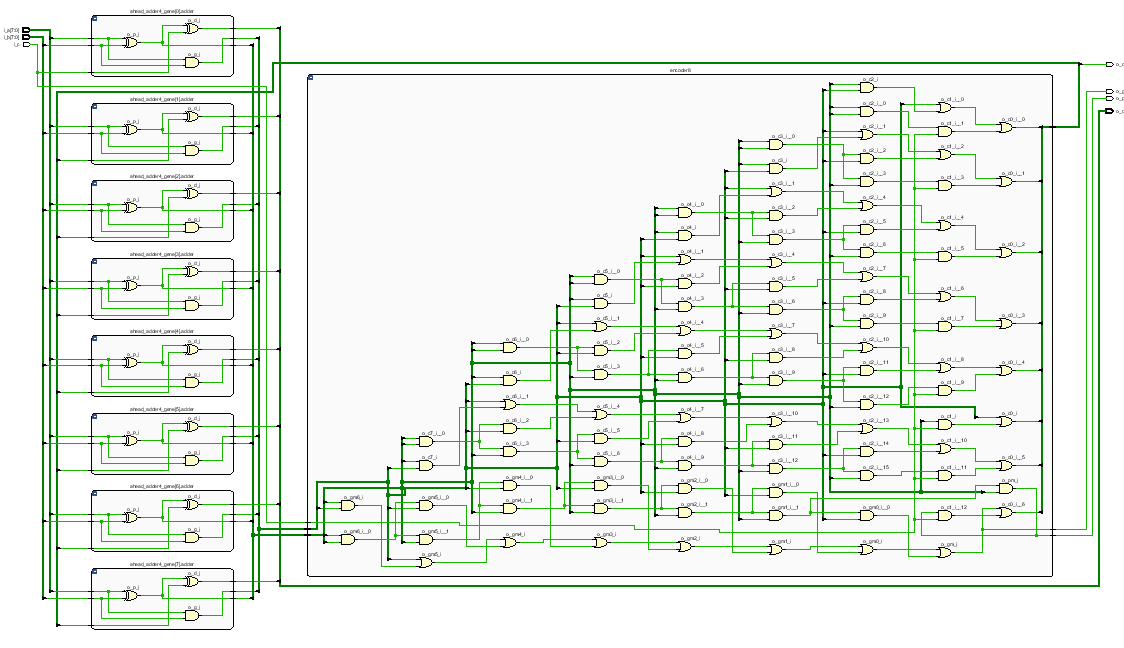
\includegraphics[width=1.0\linewidth]{rtmq/ahead_adder_8bits}
\end{figure}

\begin{figure}
    \centering
    \caption[16位超前进位加法器的FPGA实现结构图]{16位超前进位加法器的FPGA实现结构图(Vivado)\label{fig:ahead_adder_16bits}}
    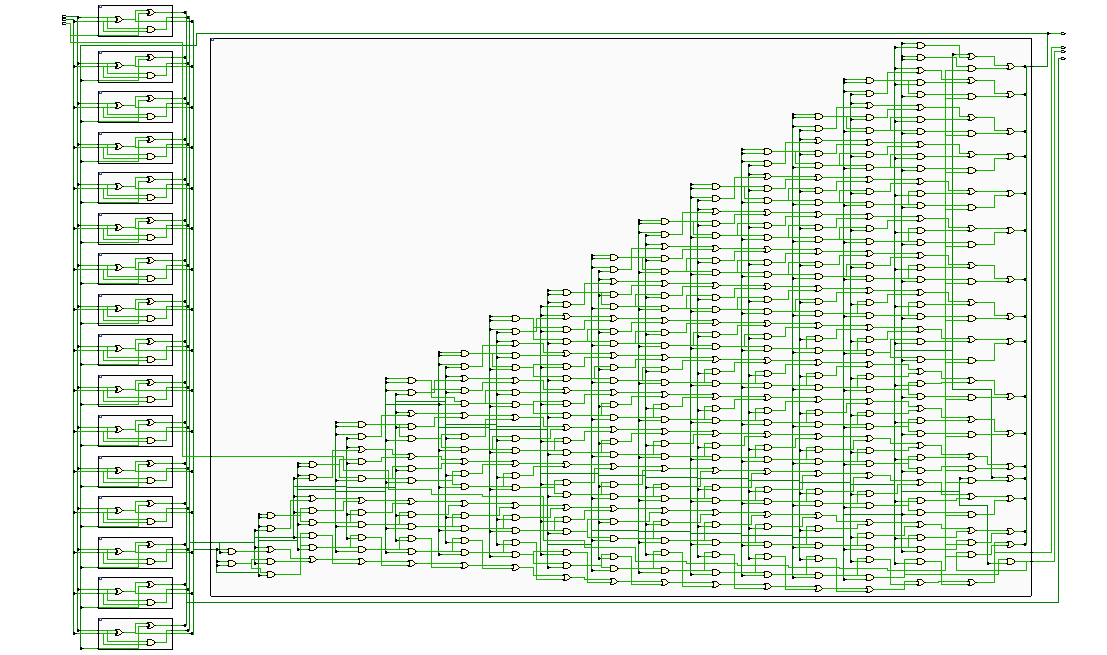
\includegraphics[width=1.0\linewidth]{rtmq/ahead_adder_16bits}
\end{figure}


\begin{figure}
    \centering
    \caption[32位Booth乘法器编码和加法树表]{32位Booth乘法器编码和加法树表\label{fig:booth_multiplier_32bits_basic}}
    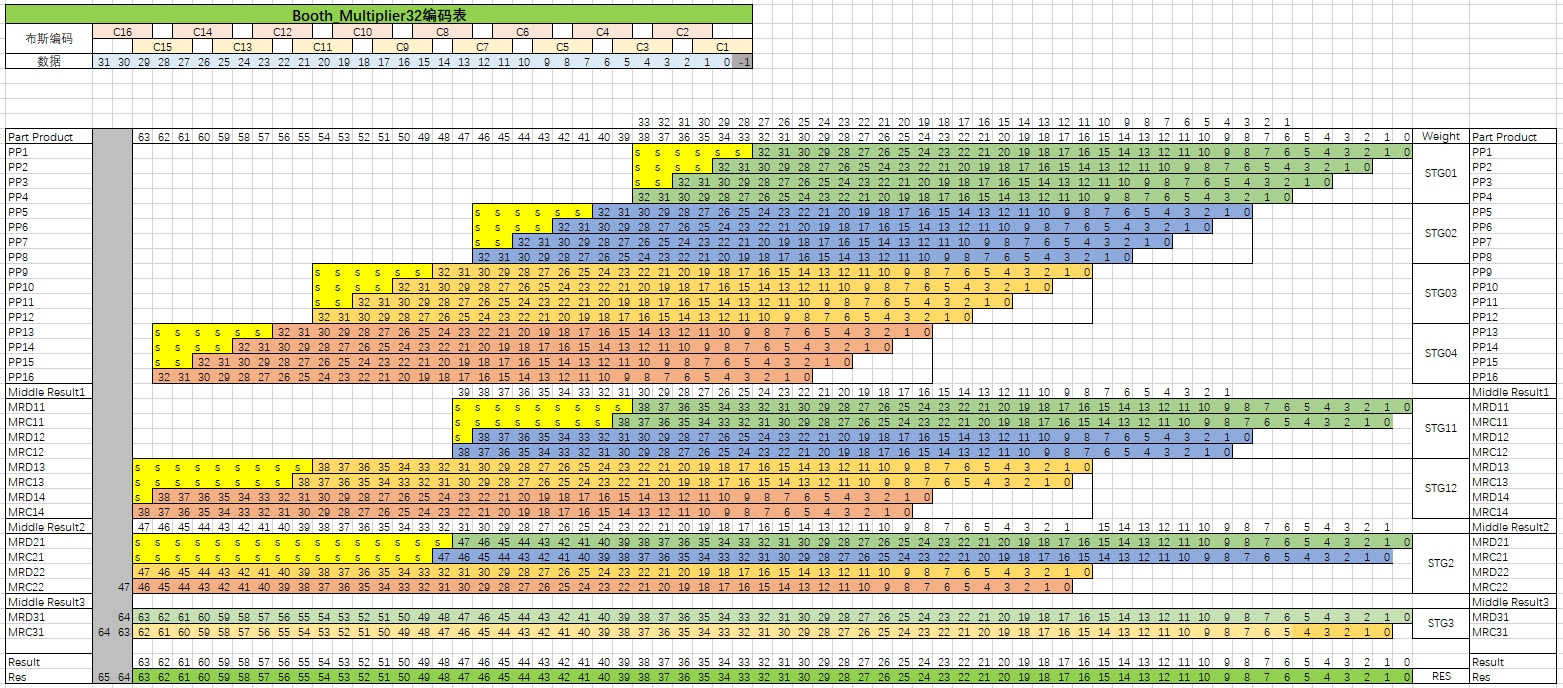
\includegraphics[width=1.0\linewidth]{rtmq/booth_multiplier_32bits_basic}
\end{figure}

\begin{figure}
    \centering
    \caption[脉冲激光拍频锁定系统图]{脉冲激光拍频锁定系统图\label{fig:beat_note_stabilization_real}}
    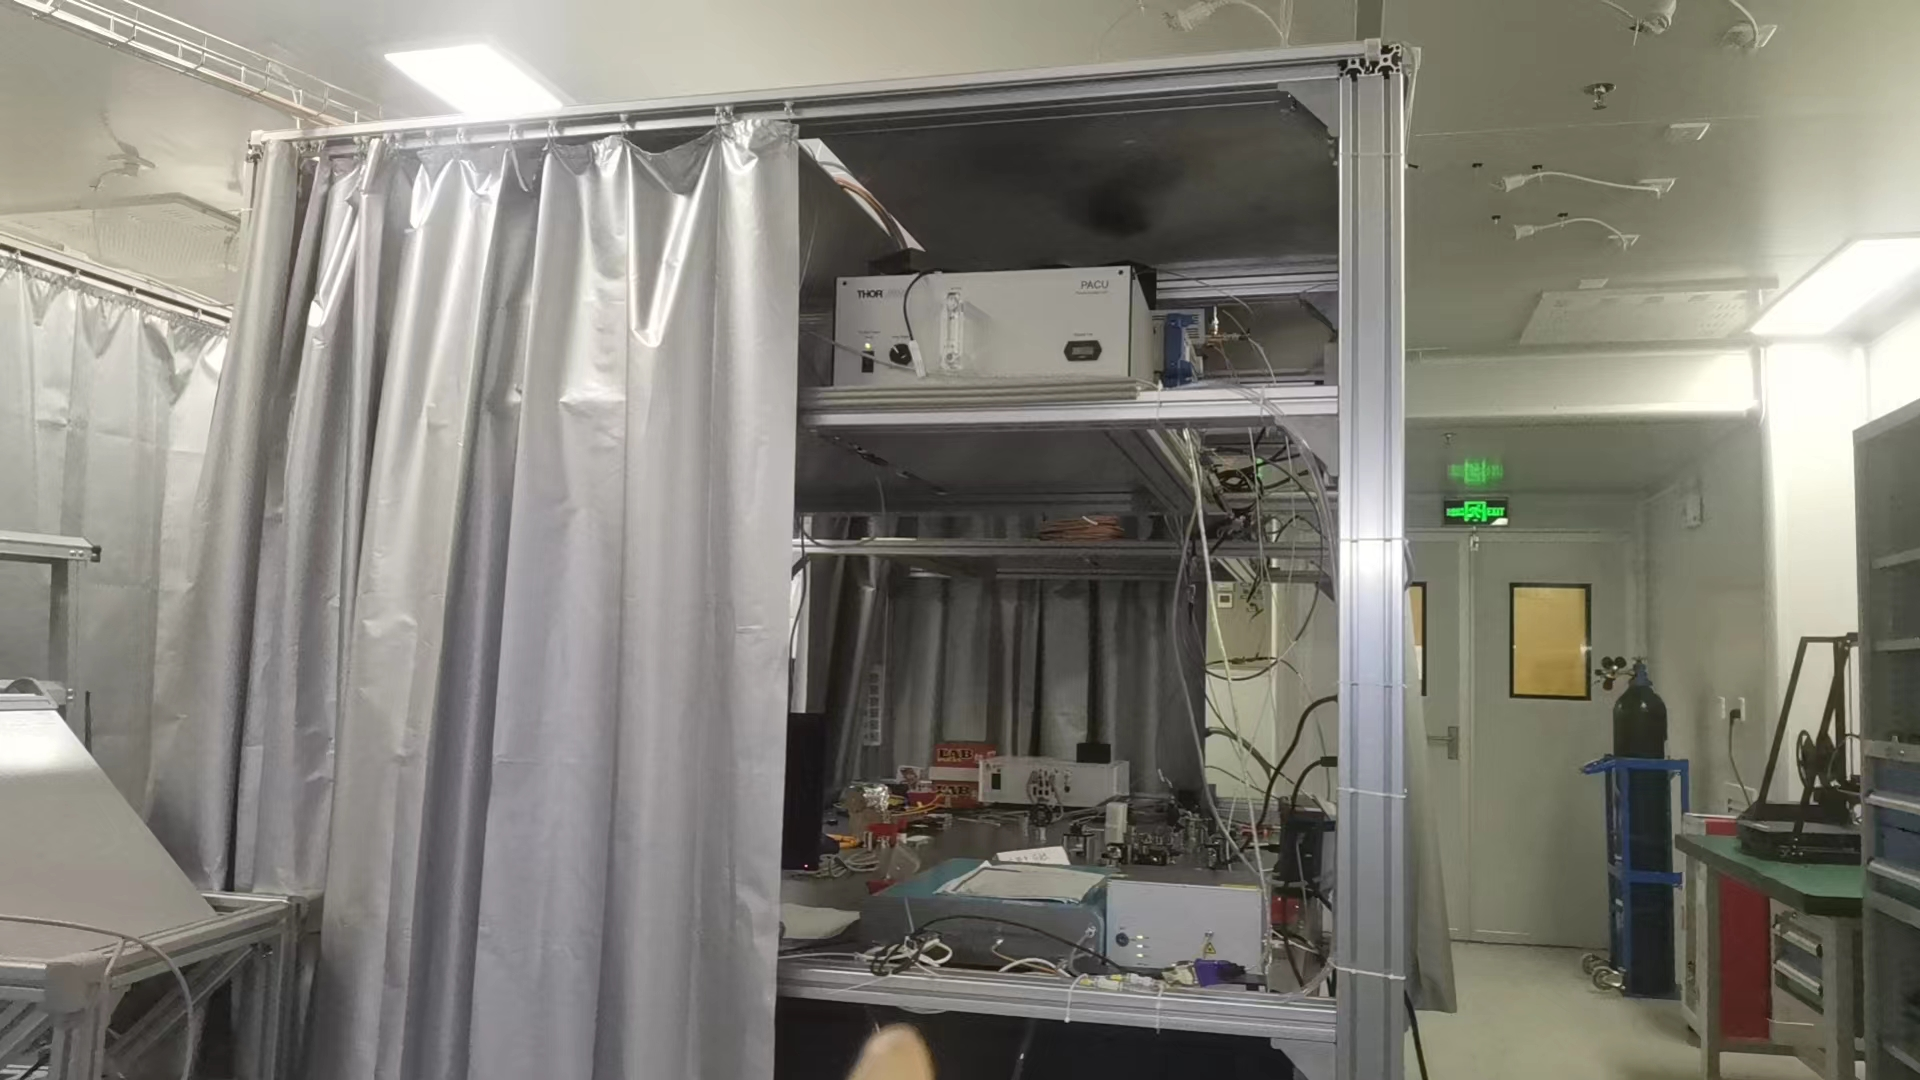
\includegraphics[width=1.0\linewidth]{beat_note_stabilization_real}
\end{figure}

\begin{figure}
    \centering
    \caption[阱频锁定模块实验测试图]{阱频锁定模块实验测试图\label{fig:trap_frequency_lock_real}}
    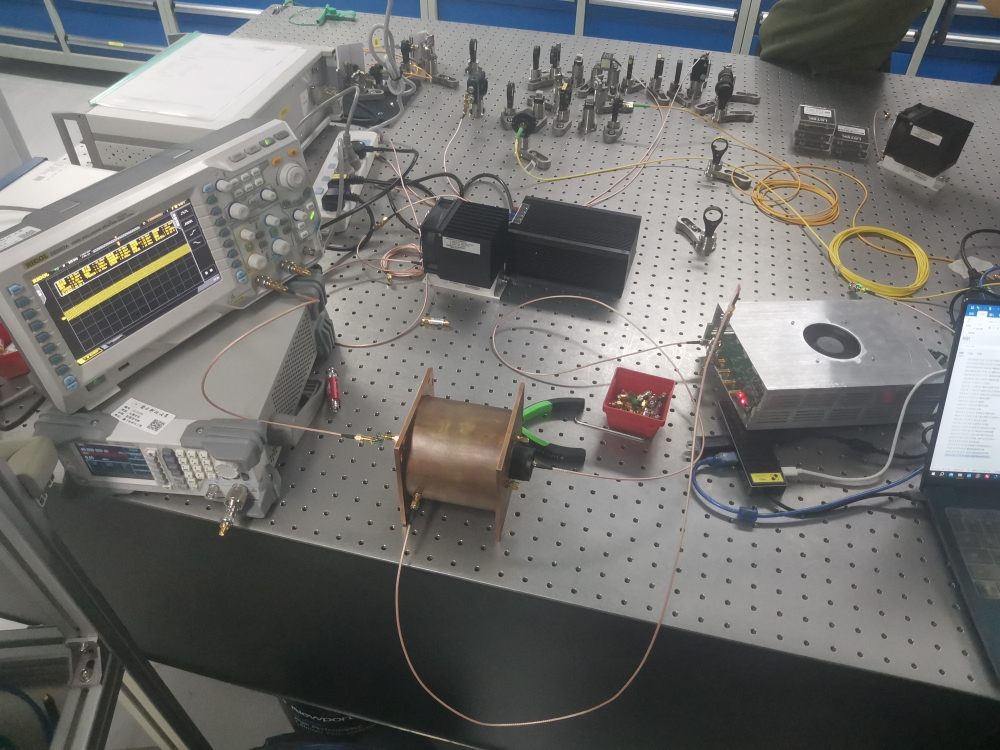
\includegraphics[width=1.0\linewidth]{trap_frequency_lock_real}
\end{figure}

\begin{figure}
    \centering
    \caption[激光功率锁定系统测试图]{激光功率锁定系统测试图\label{fig:laser_stabilization_real}}
    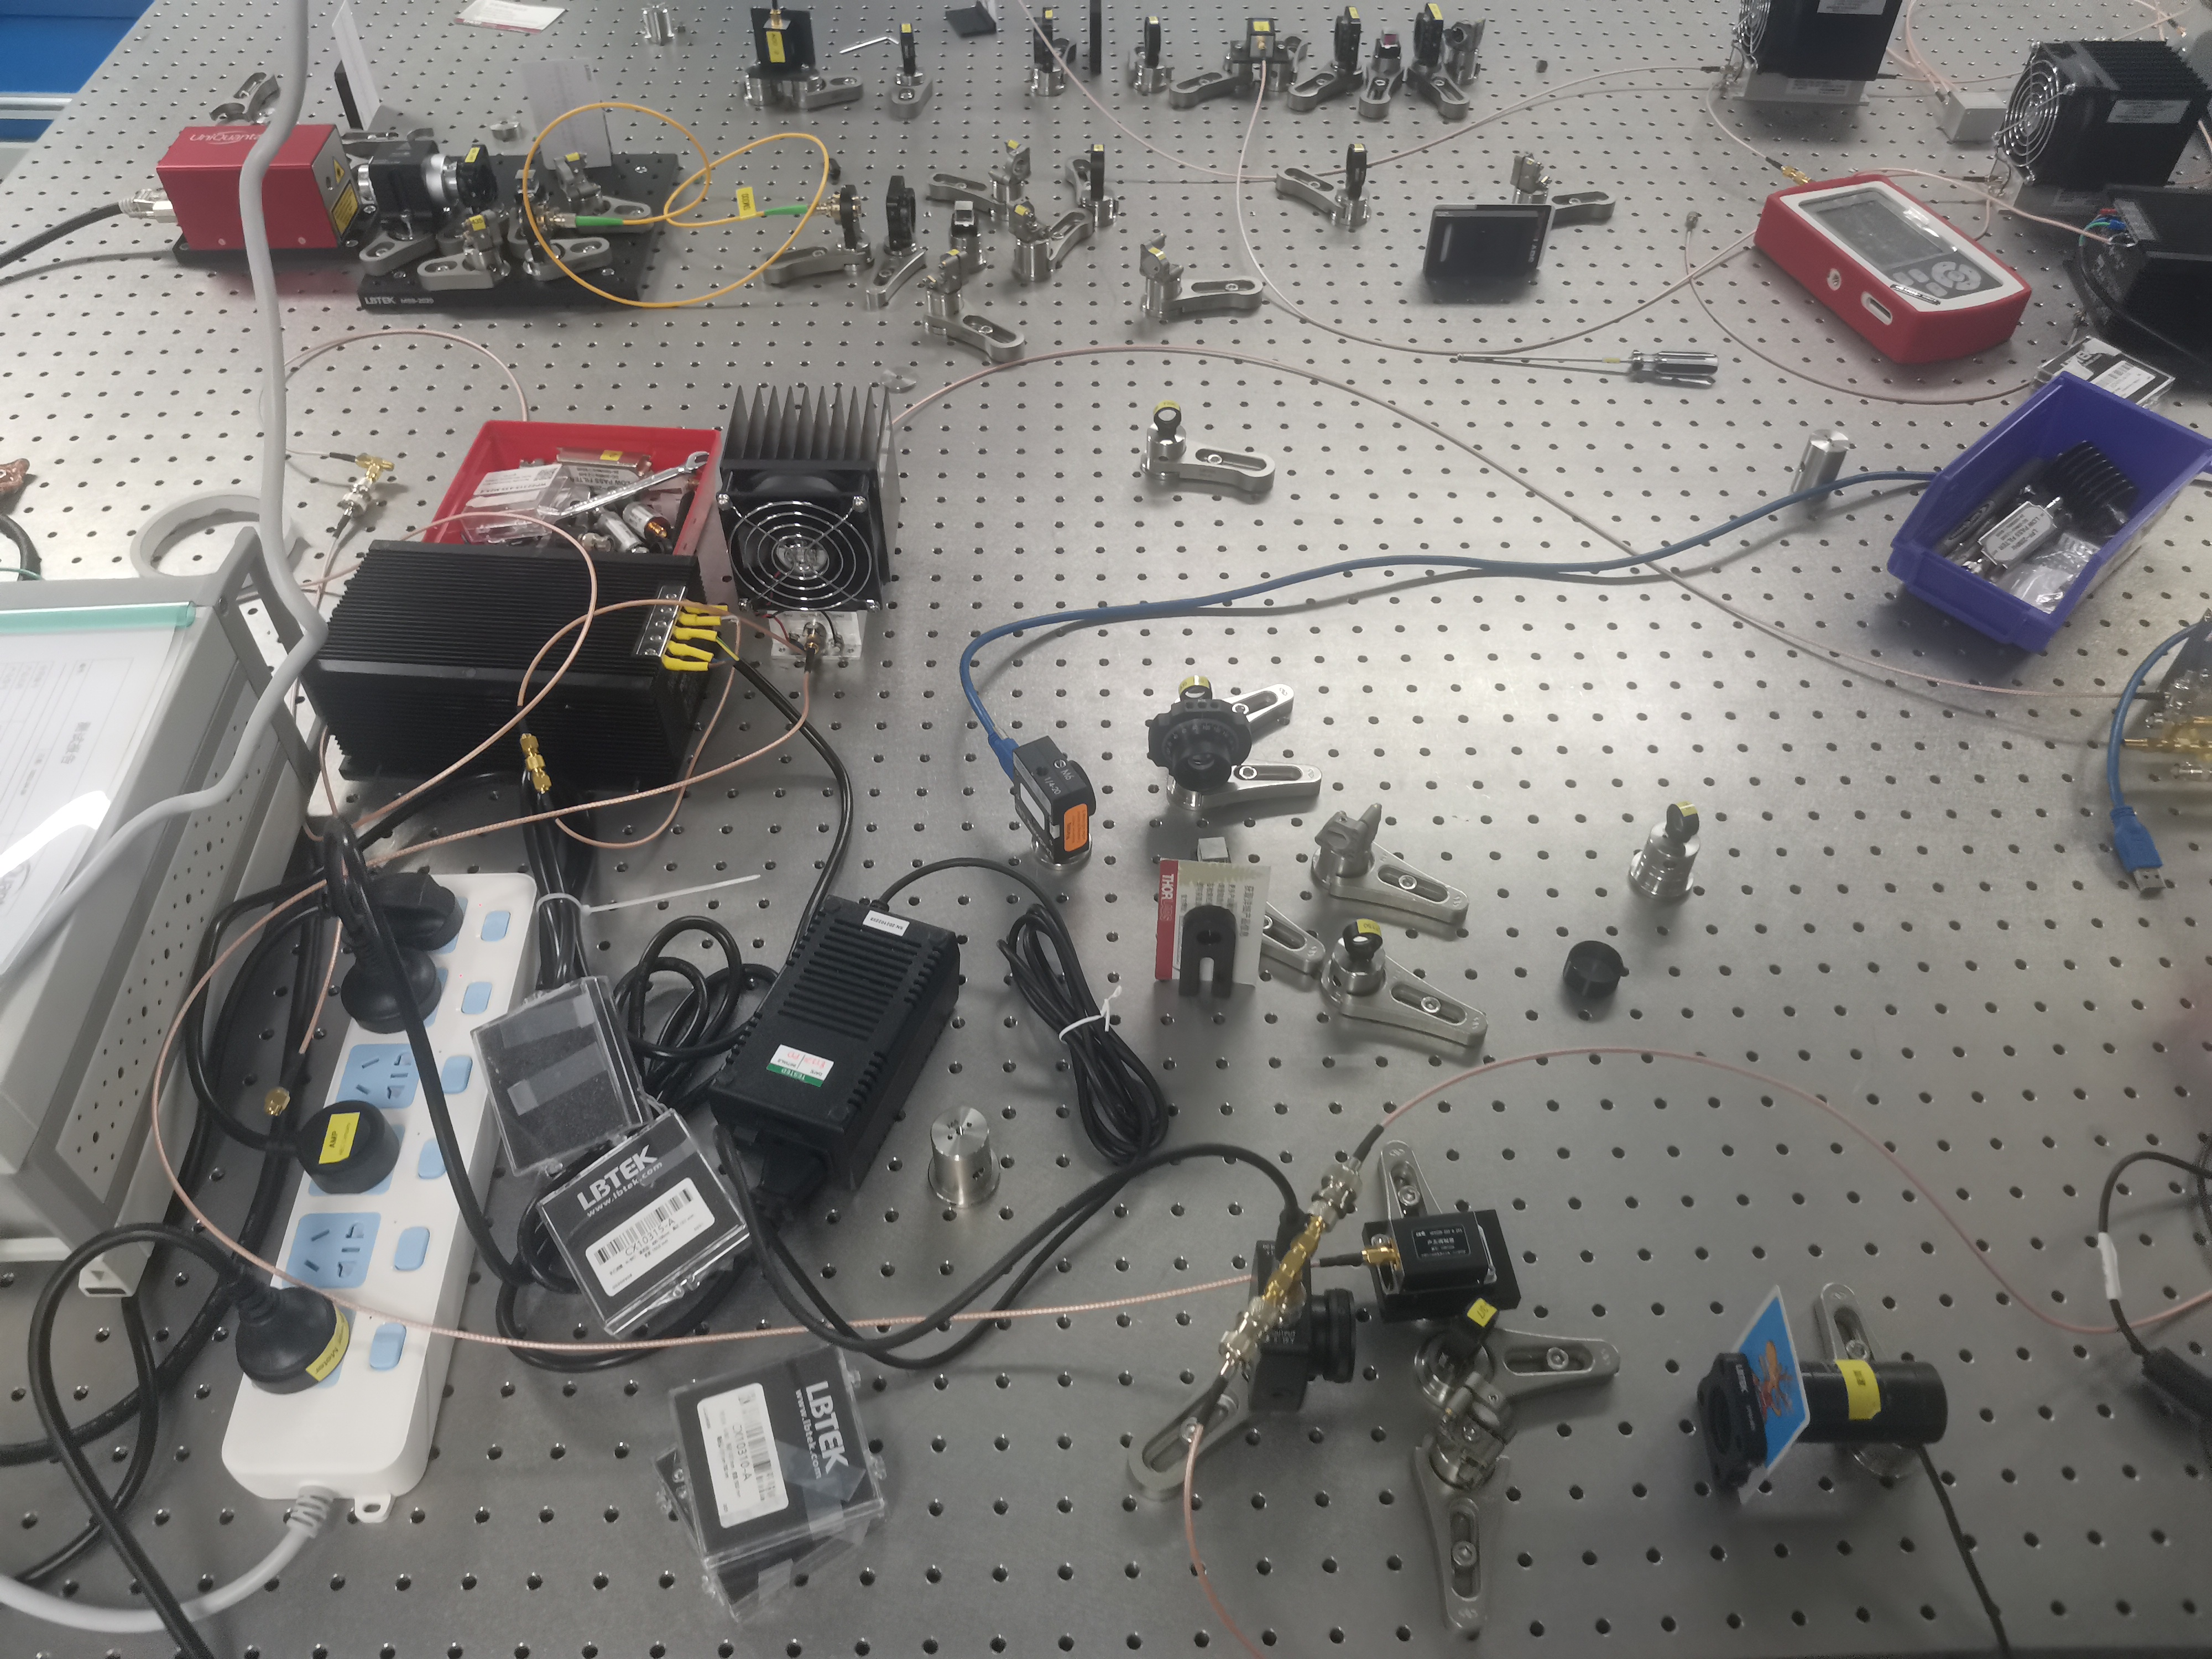
\includegraphics[width=1.0\linewidth]{laser_stabilization_real}
\end{figure}

\begin{figure}
    \centering
    \caption[激光功率外部稳定的拓展方案架构图]{激光功率外部稳定的拓展方案架构图\label{fig:laser_stabilization}}
    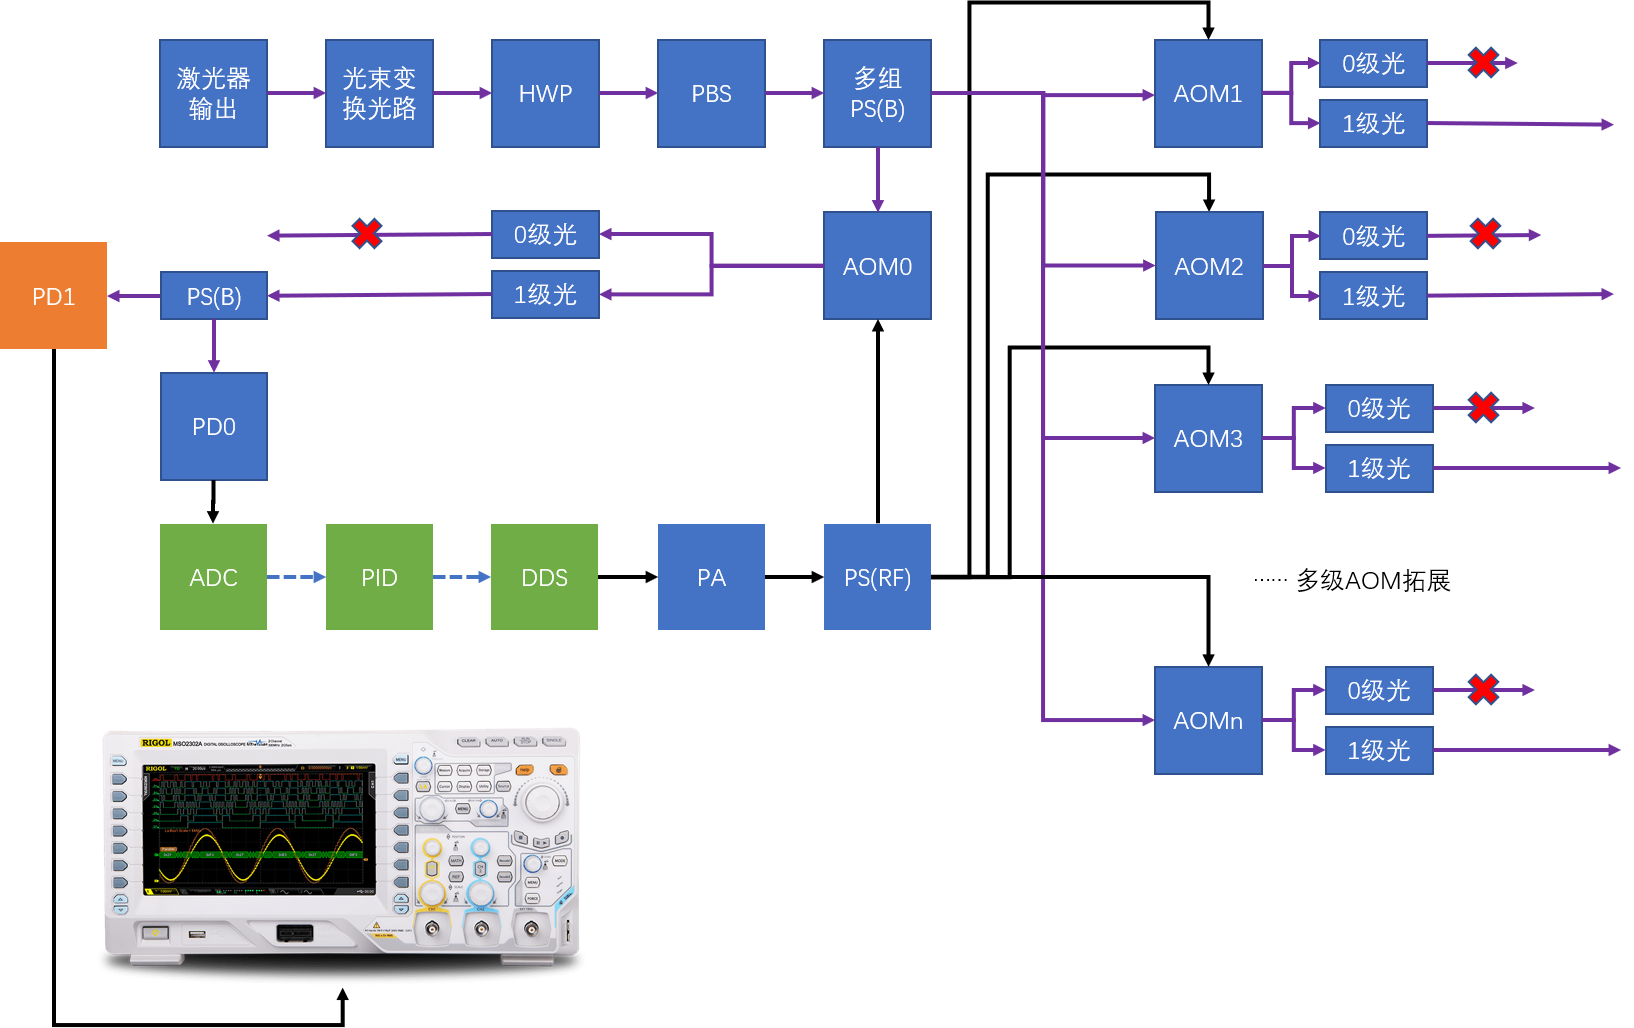
\includegraphics[width=1.0\linewidth]{laser_stabilization1}
\end{figure}

\end{document}
